\documentclass{swfuthesise}

\addbibresource{evon.bib}

\swfusetup{
  Title ={Development Aid Allocation: Building An Unsupervised Machine Learning
    Recommender System Utilizing Multidimensional Indices},%
  Author       ={MD Evon Shahriar Sohan}, % 
  Signature    ={
\includegraphics[width=5cm]{sig.pdf}}, % 作者签名(用于原创声明页)
  ID           ={201801024}, % 
  Year         ={2021},
  Month        ={December},
  Date         ={3},
  Advisor      ={Mr. WANG Xiaolin}, %
  Reviewer ={Dr. Zhenping QIANG}, % 评阅人
}

\begin{document}

\maketitle

\begin{abstract}
  Development aid or foreign assistance is the voluntary international transfer of goods,
  services, or capital resources by governments or other international aid agencies to
  support the development of recipient countries or their population. It is now one of the
  most significant factors in international relations and the national economy of many
  countries. Development aid is also one of the most researched fields in
  economics. Because well-thought-out and carefully organized aid allocations can make the
  world safer, more equal, ecologically resilient, and prosperous, which serve the aid
  contributor just as much as it benefits the aid recipient. But still, several empirical
  analysis of aid allocation confirms that donor interests continually tends to outweigh
  recipient needs. As aid allocations are national policy decisions and responsibilities,
  it leaves no room for others to suggest any obligatory aid allocation strategy. It is
  only up to the donor countries and aid agencies to include recipients when negotiating
  grants, projects, and policies, making the likelihood of attaining success in the
  Sustainable Development Goals (SDGs) solely dependent on the donor's interests. But we
  can suggest data-driven approaches keeping recipient needs in check to try to influence
  donor interests on the right track with the SDGs. We need to balance the legitimate
  interests of donors, recipients, and, most importantly, disadvantaged individuals so
  that the aims, incentives, and information of aid agents get well-aligned with the goals
  of the donors and the recipients. In this paper, we used multidimensional poverty
  measures to provide a more accurate and transparent representation of the privations
  people undergo. Because the prevailing inadequately-featured monetary indicator-based
  selection approaches significantly misidentify deprivations in other dimensions. Then
  with unsupervised machine learning techniques, we let our developed computer model
  analyze all those data without any tampering and finally recommend which countries are
  in the most desperate need of aid. Such systems can help donor countries and agencies
  efficiently allocate the bilateral or multilateral aids keeping the beneficiary's
  necessities and their targeted development goals aligned.

  \begin{keyword}
    Aid allocation; cluster analysis; unsupervised learning; multidimensional
    poverty; Sustainable Development Goals; Python; Google Colab;
  \end{keyword}
\end{abstract}

\tableofcontents % 目录
\newpage
\thispagestyle{empty}
\listoffigures
\listoftables
\listoffixmes
\clearpage
\pagenumbering{arabic}

\chapter{Introduction}

The amount of development aid given has risen in large amounts in recent decades. Official development assistance (ODA) from members of the Organisation for Economic Cooperation and Development (OECD) distributed 168 billion USD in 2019 around the world compared to 85 billion USD in 1990. Figure~\ref{fig:net} below shows the geographical distribution of aid for the
period of 1990 to 2019. 

\begin{figure}[htp]
  \centering
  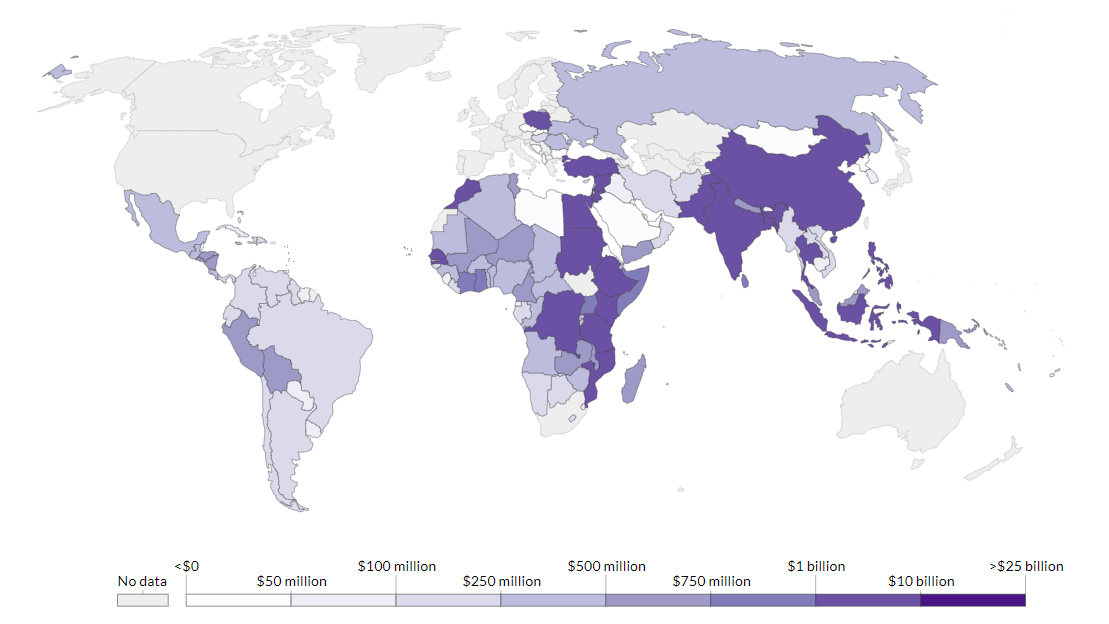
\includegraphics[width=\linewidth]{net-official-development-assistance-and-aid-received}
  \caption{Net ODA and aid received, 1990 -- 2019 (Source: The World Bank)}
  \label{fig:net}
\end{figure}
  
Such aid is now in the spotlight as never before and considered an essential factor for fulfilling Sustainable Development Goal 1, which is to end the poverty of all forms for the developing nations. But the effectiveness and impacts of development aids are still debated to this day. At present, far too much assistance is driven by geopolitical and commercial objectives rather than by efforts to protect the rights of impoverished people. Given these conditions, when the aid gets distributed in 72\% bilateral and only 28\% in multilateral channels, and that too mainly by weighing out the donor countries self-interest and the recipient countries income groups, it will surely end up vitiating the overall effectiveness of the Sustainable Development Goals (SDGs). And this is where we can step in to take some action to close the gap between the donor's interest and recipient needs.

\section{Background Information}

Rich countries are giving away more aid than at any other time on record in several forms, including humanitarian and disaster relief, economic aid to sponsor development, or investments in infrastructures, military support, healthcare programs, etc. 

Public aids such as Official Development Assistance (ODA) can be bilateral, given by the government of one country to another, such as United States Agency for International Development (USAID) or Spanish Agency for International Development Cooperation (AECID). Public aids can be multilateral too, where it gets distributed by one or many countries to or through a multilateral agency. Alternatively, aids can also be private, provided by NGOs or charity-based organizations, such as the Red Cross or Oxfam.

The motivation behind countries giving development aid can range from the most idealistic and altruistic motivations to the most cynical and strategic. But in a nutshell, nations provide foreign assistance for three main reasons. The first is for moral, ethical, or altruistic reasons. In this category, aids get distributed in compensation for past damages, exploitation, or consequences of colonialism. But the common goal remains to counter the uneven allocation of global natural or wealth resources and advance shared prosperity from the moral obligation to improve the standard of living to less fortunate people. The second reason would be economic self-interest. This form of aid gets granted to develop and expand markets for a donor country’s goods. For example, the tied aid falls in this category of assistance. It is a foreign aid that must get spent on goods or services produced in the donor country. And the third reason is political or strategic self-interest. A country provides foreign assistance to buy allies and control, mainly for security reasons like the way during the Cold War, the US used aid to incentivize countries to side with them instead of the Soviet bloc. 

Overall empirical analysis of aid allocation confirms that industrialized countries pursue development abroad when and where it serves their self-interest. And it created a raging debate around the impact of aid not only on researchers but on people of different walks of life.

\section{Literature Review}
\label{sec:lit}

The idea of development aid dates back to the early modern period of the late Middle Ages of the post-classical era in the 20th century. But the concept of development aid got huge attention after all nations committed to helping achieve the Millennium Development Goals (MDGs) by the year 2015. Since then, several empirical research projects on the distribution of development aid, including the papers that worked the period of the Cold War too, got published and confirmed the view for aid being used as a vehicle primarily for accelerating the economic and political advantages of donor states. 

Alesina and Dollar (2000)\cite{alesina2000gives} showed that aid allocation decisions used to be dictated by political and strategic considerations instead of reflecting the recipient's needs. Donor interest always seems to play a particularly significant role in aid allocation. Also, in a series of studies, Bueno de Mesquita and Smith (2007, 2009)\cite{de2007foreign}\cite{de2009political} asserted that foreign aid is a means for administrators from donor countries to acquire policy concessions from leaders in aid-receiving countries. 

Donors typically insist that their aid allocation get based on a multidimensional objective function. Yet, various developing countries, particularly in Sub-Saharan Africa, will in all likelihood miss out not only on the most prominent Sustainable Development Goals (SDGs) but also the more specific targets, e.g., those related to hunger, health, and education. Berthélemy (2006)\cite{berthelemy2006aid}, Hoeffler and Outram (2011)\cite{hoeffler2011need} argued that the allocation of aid by donor countries may reflect the economic development calls of recipient nations, but it is also getting driven by a pursuit of self-interests by donor nations. Studies from Alesina and Dollar (2000)\cite{alesina2000gives}, Knack and Rahman (2007)\cite{knack2007donor}, Djankov et al. (2008)\cite{djankov2008curse} regarded such a scenario as a constraint to the economic development of receiving countries.  

Many aid allocation studies like Jalée (1969)\cite{nuti1969pillage}, Frank (1969)\cite{frank1969underdevelopment}, Hayter (1971, 1981)\cite{hayter1971aid}\cite{hayter1981creation}, Hensman (1971)\cite{hensman1971rich}, McKinlay and Little (1977, 1978, 1979)\cite{mckinlay1977foreign}\cite{mckinlay1978foreign}\cite{mckinlay1979aid}; Maizels and Nissanke (1984)\cite{maizels1984motivations}, McGillivray (2003)\cite{mcgillivray2003aid}; Feeny and McGillivray (2002)\cite{feeny2002modeling}, Berthélemy and Tichit (2002)\cite{berthelemy2002bilateral}, Harrigan and Wang (2011)\cite{harrigan2011new} that used models which incorporate variables representing both donor interest and the recipient need have also concluded that in the geographic distribution of aid, donor interest plays a significant role, especially on the part of bilateral donors. In particular, McKinlay and Little’s (1977, 1978)\cite{mckinlay1977foreign}\cite{mckinlay1978foreign} studies have found that humanitarian criteria did not significantly affect U.S., U.K. or French aid flows to non-communist countries during the Cold War. Instead, they were likely driven by foreign policy concerns and an increase in trade for the donor countries. Tammy L. Lewis’s (Vol. 84, No. 1, 2003)\cite{lewis2003environmental} affirmed that environmental aid donors prefer countries with whom they have had former relations e.g. in economic and security, or countries that are democratic, or countries that have unexploited natural resources. In short, donor interests surpass recipient needs in almost all cases. 

Papers from the Review of World Economics 2007, Vol. 143, No. 4, especially the Thiele et al. (2007)\cite{thiele2007donors} research studied the aid portfolio and the target of various bilateral and multilateral donors and found some possible cause behind this development aid failure, namely that donors may have paid insufficient attention to the MDGs by not allocating aid according to the MDG-related needs of recipients, and inadequately poor targeting of aid. 

Ruggeri-Laderchi, Saith, and Stewart (2003)\cite{laderchi2003does} observed that in India, around half of the children and more than half of adults who were capability poor according to the education or health as the indicator, were not in monetary poverty; similarly, more than half of the nutrition-poor children were not in monetary poverty. Traditional monetary poverty indicators appeared to be significantly misidentifying deprivation in other dimensions of need. 

Economists such as McGillivray (2003)\cite{mcgillivray2003aid} and Amprou et al. (2007)\cite{amprou2007aid} have called for a more progressive concept of aid allocation. Because the selection of aid beneficiaries only by embracing the income and policy situation of recipient countries as proposed by Collier and Dollar (2002)\cite{collier2002aid} is not the proper solution. 

Therefore, if we consider poverty only by calculating the monetary indicators such as the amount of income-deprived people then a large proportion of impoverished people that are facing hardships on other dimensions are going to be left behind. That's why we need to develop a system that can be used to measure the complex multidimensional aspects of poverty worldwide using computing resources to help those who are in direst need of aid and let donors allocate aids in a way that will also sync with the goals of SDGs.


\section{Research Problem}

As we've seen in the literature review section (Section~\ref{sec:lit}) that an immense amount
of empirical study got published since the inclusion of development aid as the eighth goal
of the Millennium Development Goals (MDGs). All those studies unveiled the complex
economic environment, both at the national and international levels within which aid
operates. And the existing works confirm that aid increases alone will not help reduce the
suffering of the disadvantaged or achieve the Sustainable Development Goals (SDGs) without
bringing significant improvements in the quality of that aid. Also, global prosperity will
be hard to achieve until we close the distant relationships between the donors and
beneficiaries. And to solve this centuries-long dilemma, we need to employ
multidimensional measures to design a system that can recommend the regions or populations
in the direst need of aid based on all the different factors and gathered data we put in
it. Once done, the solution can help get recipient needs acknowledged by letting the contributors make informed decisions on aid allocation, thus will keep both the recipient and donor needs and objectives aligned with the SDGs.

\section{Objectives}

The connection between aid allocation theories and practice in the field has not been aptly experimented with to measure the efficacy of our current distribution techniques. It is necessary to pursue that kind of analysis for remodeling the allocation strategies to get better results from both the donor's and recipient's prospects. So, to eradicate global poverty and ensure economic growth, we must move from theory to applications to accurately address the multi-layered factors that influence aid effectiveness. Therefore, considering the limitations of current aid allocation methods, analysis of clustering of the recipient countries by aid-relevant multidimensional indicators might have the potential to highlight and develop pragmatic policy proposals.

\chapter{Materials}

All the multidimensional measures we’ve used in this research are from open-access databases of recognized platforms, such as the Oxford Poverty and Human Development Initiative's (OPHI) Global Multidimensional Poverty Index (MPI), World Bank national accounts data files, and the OECD National Accounts Statistics dataset. And we analyzed, studied, and designed our recommender model from these diverse datasets inside Google's cloud-based Colaboratory Jupyter notebook using the Python programming language.

\section{Multidimensional Indices}

Achieving a better and more sustainable future for all humans encompasses multiple aspects of life, including being free, healthy, educated, employed, and many other interlinked vital factors for relishing fulfillment.

And to bring that into the world, we can't keep making aid allocation decisions using the conventional monetary indicators alone, assuming that these indicators will be good enough for understanding multidimensional poverty. It's because it'll be the same as presuming that consumption poor people are equal to those who suffer diseases, malnutrition or similar to those who are uneducated, helpless, or disempowered.

That's why we need to look at the problem from multidimensional prospects because the more dimensions used in a query, the better the retrieval performance. We must gather a multi-field index that will contain multiple features to reveal the poverty dimensions properly so that the system behaves like a virtual cube of values that can precisely intersect at measures of interest.

\subsection{Data Collection}

We've collected our data from distinct reputable and authentic sources, as shown in
Figure~\ref{fig:multidimensional}. That diagram gives a schematic representation of our
data sources and features.

\begin{figure}[!htp]
  \centering
  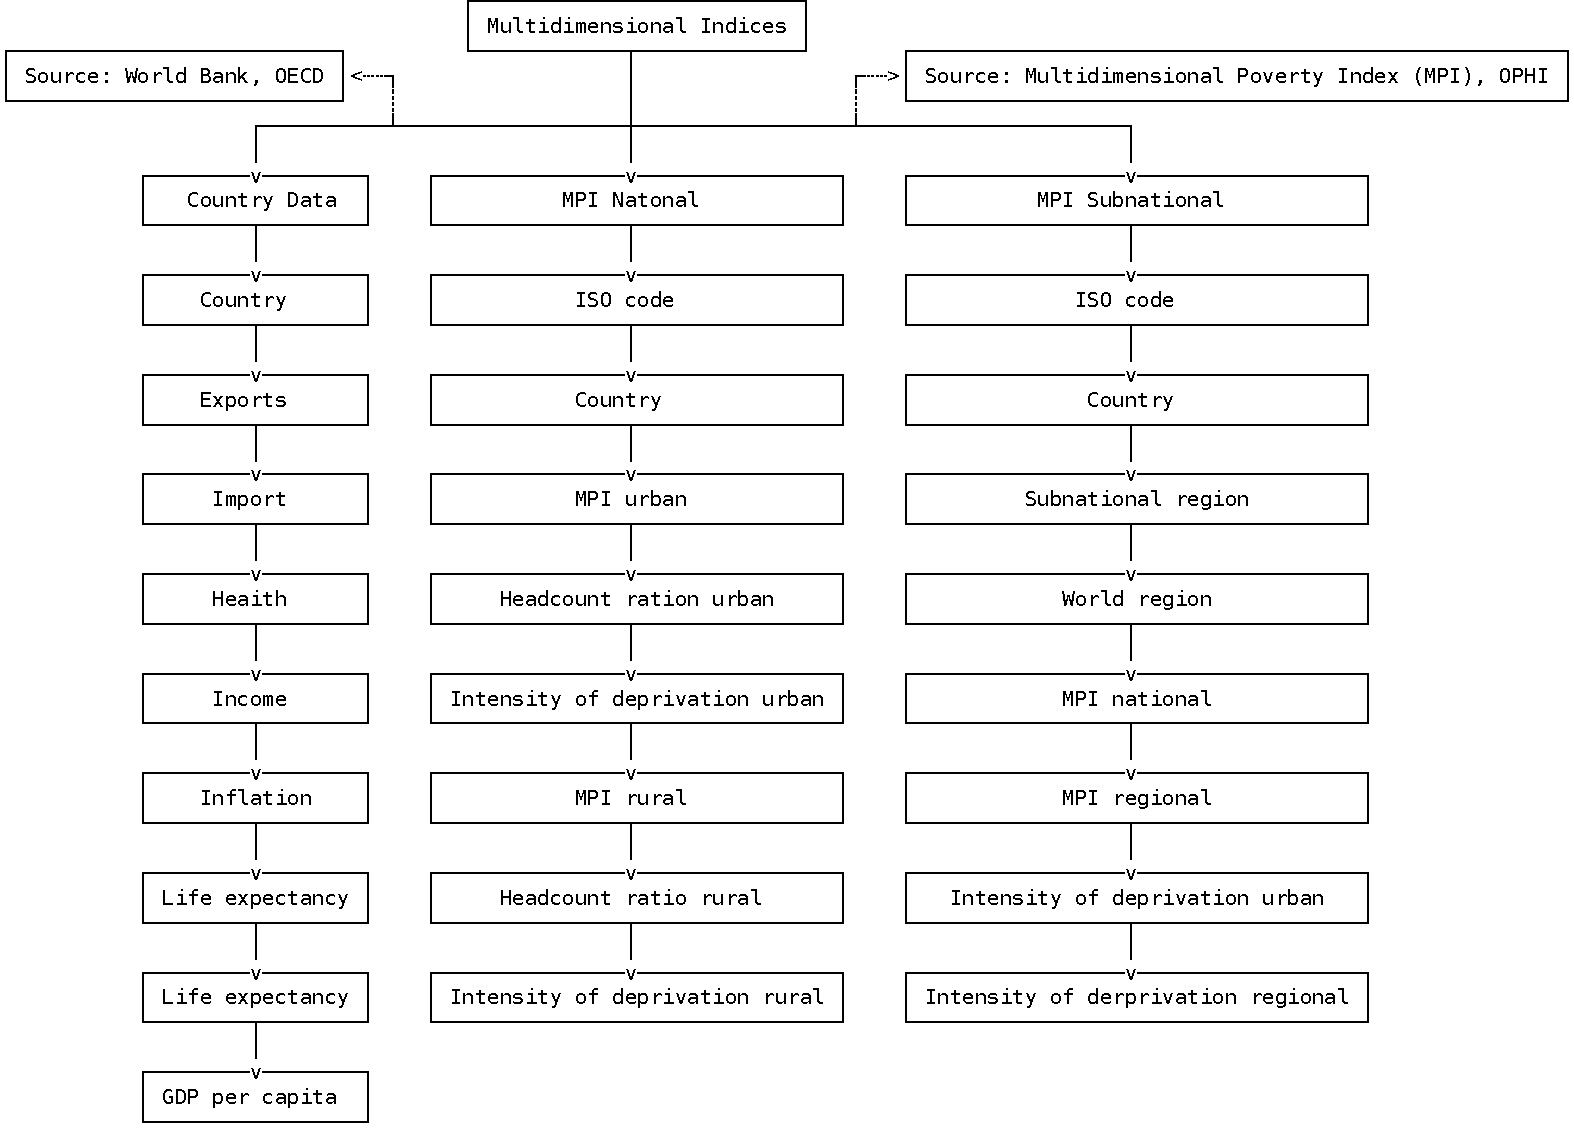
\includegraphics[width=\linewidth]{figs/multidimensional-indices}
  \caption{Multidimensional measures used in this study}
  \label{fig:multidimensional}
\end{figure}

\subsubsection{Country Data}

This dataset includes multidimensional indicators sourced from the World Bank and OECD
National Accounts data files for 167 countries. In Table~\ref{tab:country}, we displayed the first ten rows to show the existing features and values for this particular dataset.

\begin{table}[!ht]
  \centering%
  \caption{Country data sample rows (Source: Compiled from the World Bank and OECD)}%
  \label{tab:country}%
  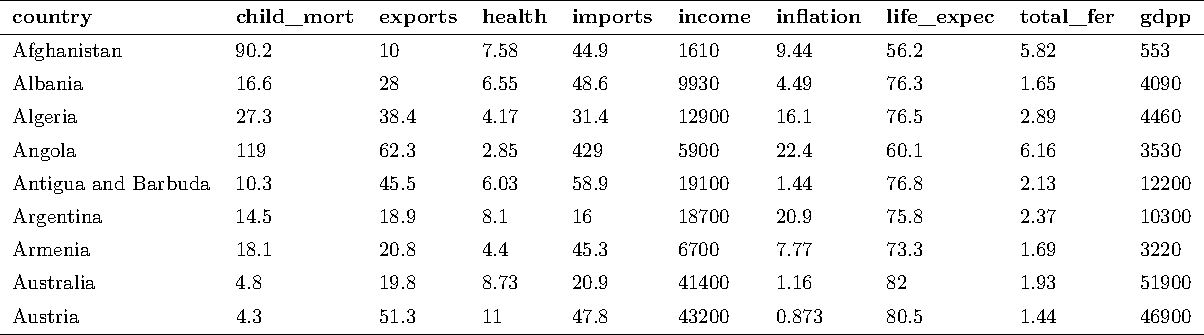
\includegraphics[width=\linewidth]{country_data}
\end{table}
  
\paragraph{World Bank Data}

The World Bank is an international organization owned by 187 member nations that share data and statistics for over 200 countries with 1200 indicators on development topics. Their development indicators and visualization engines get compiled from well-known and officially recognized international sources. That's what makes the data present the most recent and accurate global development data, including the national, regional, and global estimates for an out-and-out detailed analysis.

\paragraph{OECD National Accounts Statistics}

The Organisation for Economic Co-operation and Development (OECD) is a global policy forum with developed nations as members, participating in the shared goal of advancing balanced, robust, cleaner economic growth worldwide. Their national accounts statistics data files hold annual and quarterly data of various monetary indicators for OECD and non-member countries' economies. Their database has expenditure-based, output-based, and income-based gross domestic product (GDP); population and employment records; GDP per capita; disposable income; general government accounts; PPPs and exchange rates; financial flows, stocks, and central government debts of countries from all around the world.

The features used in these datasets are listed below with their initial descriptions.

\begin{description}
\item[country:] Name of the country.
\item[child\_mort:] Death of children under five years of age per thousand live births.
\item[exports:] Exports of goods and services per capita (\% of GDP).
\item[health:] Total health expenditure per capita (\% of GDP).
\item[import:] Imports of goods and services per capita (\% of GDP).
\item[income:] Net income per person.
\item[inflation:] The measurement of the annual growth rate of the total GDP.
\item[life\_expec:] The average number of years a newborn is supposed to live if the current mortality pattern remains the same in the future.
\item[total\_fer:] The number of children is supposed to be born to each woman if the current age-fertility rate stays constant in the future.
\item[gdpp:] GDP per capita is gross domestic product divided by midyear population.
\end{description}

\subsubsection{Multidimensional Poverty Index (MPI)}

The Global Multidimensional Poverty Index (MPI) published by the Oxford Poverty and Human Development Initiative (OPHI) measures the multidimensional nature of poverty in over 100 countries.

\paragraph{Oxford Poverty and Human Development Initiative (OPHI)}

OPHI is an economic research center from the University of Oxford, established in 2007, publishing the global Multidimensional Poverty Index (MPI) annually since 2010. They do it for the United Nations Development Programme (UNDP) to help them combine the incidence and the intensity of poverty in their Human Development Report (HDR). Their goal is to build a more systematic, economic, and methodological framework for diminishing poverty on a multidimensional scale. While doing the assessments for the MPI, OPHI aims to measure the non-income-based dimensions of poverty compared to the monetary indicators to provide a more thorough and accurate evaluation of the degree of deprivations. In the MPI, people are considered poverty-stricken by measuring the intensity of the average number of weighted deprivations they experience; mainly, if they get deprived of one-third or more of the indicators shown in Figure~\ref{fig:mpi}.

\begin{figure}[!htp]
    \centering
    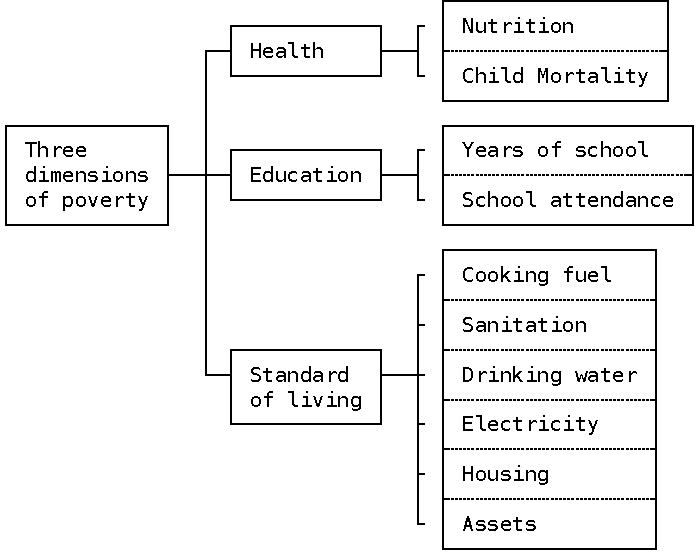
\includegraphics[width=.6\linewidth]{structure-of-the-global-mpi}
    \caption{Structure of the global Multidimensional Poverty Index (Source: OPHI 2018)}
    \label{fig:mpi}
\end{figure}

By exploring the global MPI data, we can unveil insights into diverse aspects related to global poverty, including child poverty, different geographical dis-aggregations, urban/rural demographics, etc. The MPI goes hand in hand with prevalent measures of financial poverty, such as the World Bank's extreme poverty line of \$1.90 a day\cite{world2020poverty}, by addressing the severe shortcomings in health, education, and living standards that one experiences at the same time. The MPI can help us find asymmetries at the sub-national, national, regional, and global levels. In doing so, each layer of analysis reveals a new understanding of inequality and provides a much richer picture than the poverty rate of \$1.90 per day.

\paragraph{National}

This derived dataset from the MPI holds updated data covering more than 5 billion
people. As shown in Table~\ref{tab:national}, it comprises disaggregation by age-groups, rural-urban areas, and subnational regions from 102 countries.

\begin{table}[ht]
  \centering
  \caption{MPI national data sample rows (Source: OPHI)\label{tab:national}}
  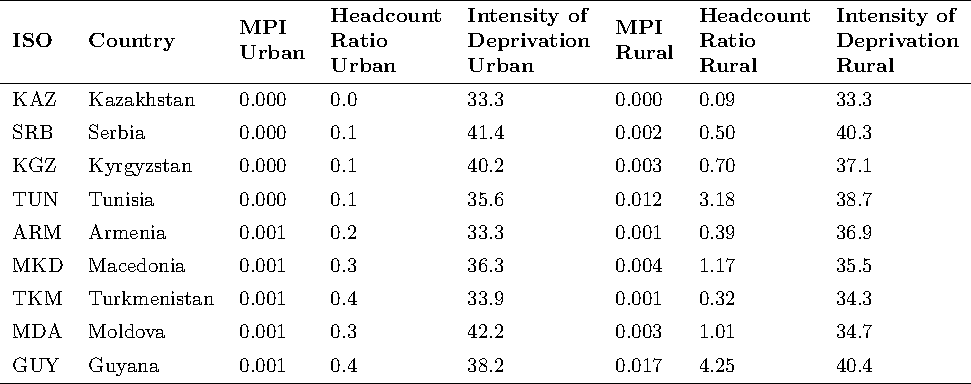
\includegraphics[width=\linewidth]{mpi_national}
\end{table}
  
The features of this dataset are listed below with descriptions.%in Table~\ref{tab:mpi}
\begin{description}
\item[ISO:] Unique ID for the country.
\item[Country:] Name of the country.
\item[MPI Urban:] Multidimensional Poverty Index (MPI) for urban areas within the country.
\item[Headcount Ratio Urban:] Poverty headcount ratio (\% of the population listed as poor)
  within urban areas within the country.
\item[Intensity of Deprivation Urban:] Average distance below the poverty line of those
  listed as poor in urban areas.
\item[MPI Rural:] Multidimensional Poverty Index (MPI) for rural areas within the country.
\item[Headcount Ratio Rural:] Poverty headcount ratio (\% of the population listed as poor) within rural areas within the country.
\item[Intensity of Deprivation Rural:] Average distance below the poverty line of those listed as poor in rural areas.
\end{description}

\paragraph{Subnational}

This dataset possesses subnational level data for each country covered in the MPI database. In Table~\ref{tab:subnational}, we can see the first ten rows of this extracted dataset with its features. 

\begin{table}[ht]
  \centering
  \caption{MPI subnational data sample rows (Source: OPHI)\label{tab:subnational}}
  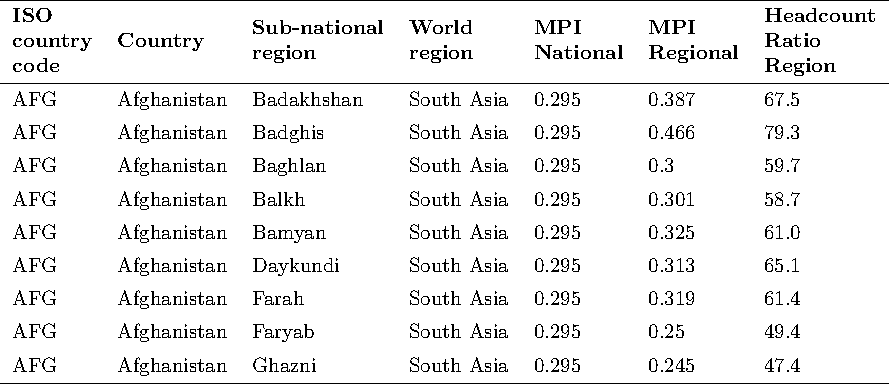
\includegraphics[width=\linewidth]{mpi_subnational}
\end{table}

And features found in this dataset are enumerated below with their elementary descriptions.

\begin{description}
\item[ISO:] Unique ID for the country.
\item[Country:] Country name.
\item[Sub-national region:] The region within the country.
\item[World region:] General global region.
\item[MPI National:] Overall aggregate national Multidimensional Poverty Index (MPI) score.
\item[MPI Regional:] Multidimensional Poverty Index (MPI) for this region.
\item[Headcount Ratio Regional:] Poverty headcount ratio (\% of the population listed as poor) in this region.
\item[Intensity of Deprivation Regional:] Average distance below the poverty line of those listed as poor in this region.
\end{description}

\section{Build Environment}

We used the Python programming language in the Google Colab cloud platform. It's because the complex algorithms and versatile workflows of machine learning techniques can stand behind the efficient Google computing resources, and Python's simplicity will let us write reliable systems so that any developer or researcher can later understand the code and upgrade.

\subsection{Google Colab}

Google Colaboratory or shortly Google Colab is a service from Google Research. This widely popular Jupyter Notebook-based cloud service allows people to write and execute Python code through the browser without requiring any additional setup. It is an excellent and well-suited tool for machine learning and data analysis tasks. We've used this platform for our project because it offers an outstanding free version of Google computing resources, such as Graphical Processing Units (GPUs) and Tensor Processing Units (TPUs). This platform enables everyone, especially researchers and data scientists, to build and collaborate on projects that blend live code, equations, computational outputs, and other multimedia resources, along with explanatory texts in a single document.

\subsection{Libraries}

A robust set of libraries, especially the open-source ones, are an essential part of a researcher's arsenal to analyze, write and develop complex programs while saving themselves from writing a lot of arbitrary code. Down below, we've cited twelve such open-source libraries used in conducting this study.

\begin{description}
\item[os] The os module provided a compact way of using diverse interfaces of an operating
  system, such as showing the absolute path of a file, current working directory, listing
  all the files in a directory, removing them, accessing or changing environment
  variables.
\item[NumPy] NumPy library made it simple to implement a number of important mathematical
  and logical operations on arrays. NumPy uses much less memory to store data with the
  help of its simultaneously compact, powerful, and expressive syntaxes.
\item[pandas] pandas library made data manipulation and analysis straightforward by
  offering powerful, expressive, and flexible data structures. It is built over the NumPy
  module that can be efficiently used in the field of computing, data analysis,
  statistics.
\item[Seaborn] Seaborn library offered a high-level interface for exploratory data
  analysis, distribution plotting, and informative statistical visualization. It uses
  Matplotlib underneath to plot graphs and is also closely integrated into the data
  structures from pandas.
\item[Matplotlib] Matplotlib is a comprehensive library for interactive visualization in
  Python, and a viable open-source alternative to MATLAB. It helped us create static,
  interactive, and animated plotting in Python 2D plots of arrays effortlessly.
\item[scikit-learn] scikit-learn is a machine learning library for Python that provides a
  range of unsupervised and supervised learning algorithms. We used it for tasks such as
  clustering, cross-validation, dimensionality reduction, feature extractions.
\item[Yellowbrick] Yellowbrick library offered visualization and diagnostic tools that
  combine the cores of matplotlib and scikit-learn. It helps the model with the algorithm
  selection process and hyperparameter tuning.
\item[GeoPandas] GeoPandas mixes the features of pandas, Shapely, and Fiona packages and
  made working and manipulating geospatial data in Python relatively easy by promoting
  spatial operations on geometric types.
\item[Geoplot] Geoplot is a graphing package that was built over the cartopy and
  matplotlib library. It helped us create nice-looking geospatial maps populated with
  data.
\item[mapclassify] We have used mapclassify, a part of the Python Spatial Analysis Library, as our Choropleth map classification engine. 
\item[Plotly] Plotly is a very useful graphing or plotting library supporting more than
  fifty unique chart types. This library makes interactive, quality graphs that cover a
  wide range of geographic, statistical, and scientific 3D use-cases.
\item[statsmodels] This Python module for statistics provided us with the classes and functions for plotting residual plots in our regression analysis.  
\end{description}

\chapter{Methodology}

To solve the proposed research problem, we have utilized our datasets with state-of-the-art unsupervised machine learning techniques. But before that, we must understand the data we're dealing with and design sophisticated data preprocessing, analyzing, and modeling stages.

\section{Understanding the Data}

To begin the study, we must understand the data at hand before we preprocess it. Because without being informed of the features, facts, figures, and distributions in the data, we can't decide on the subsequent steps necessary to back our study. Once we have some initial understanding of the data and have eliminated all the bad or poor quality data, we can start with the analysis to explore and interpret the data in meaningful ways. Because without going through the data preparation stages, there always remains a probability that the data might alter the accuracy of insights or show incorrect results due to junk data, calibration issues, or discrepancies between datasets. And performing the data analysis stage expeditiously can enable us to interpret the data without leaving anything out and derive insights by employing complex algorithms.

\subsection{Data Distribution}

Prior to applying any machine learning algorithm, we must study the underlying data distributions in a dataset because every single machine learning algorithm has a certain number of assumptions on the data. Data distribution is a listing that visualizes how often each value occurs by calculating all the possible values or intervals in the dataset. We have used histograms to see such visual interpretation of numerical data. The histogram is a graph bar for frequency distributions that shows the number of data points falling within a specified range of values. For example, in the plotted histograms below in Figure~\ref{fig:distribution}, the X-axis reveals the intervals, and the Y-axis presents the number of times the values occurred within those intervals. The bar height shows the number of times values occur within those intervals, and the width shows the covered X-axis intervals. And the attached titles are simply reporting the information included in the respective histograms.

\begin{figure}[!htp]
    \centering
    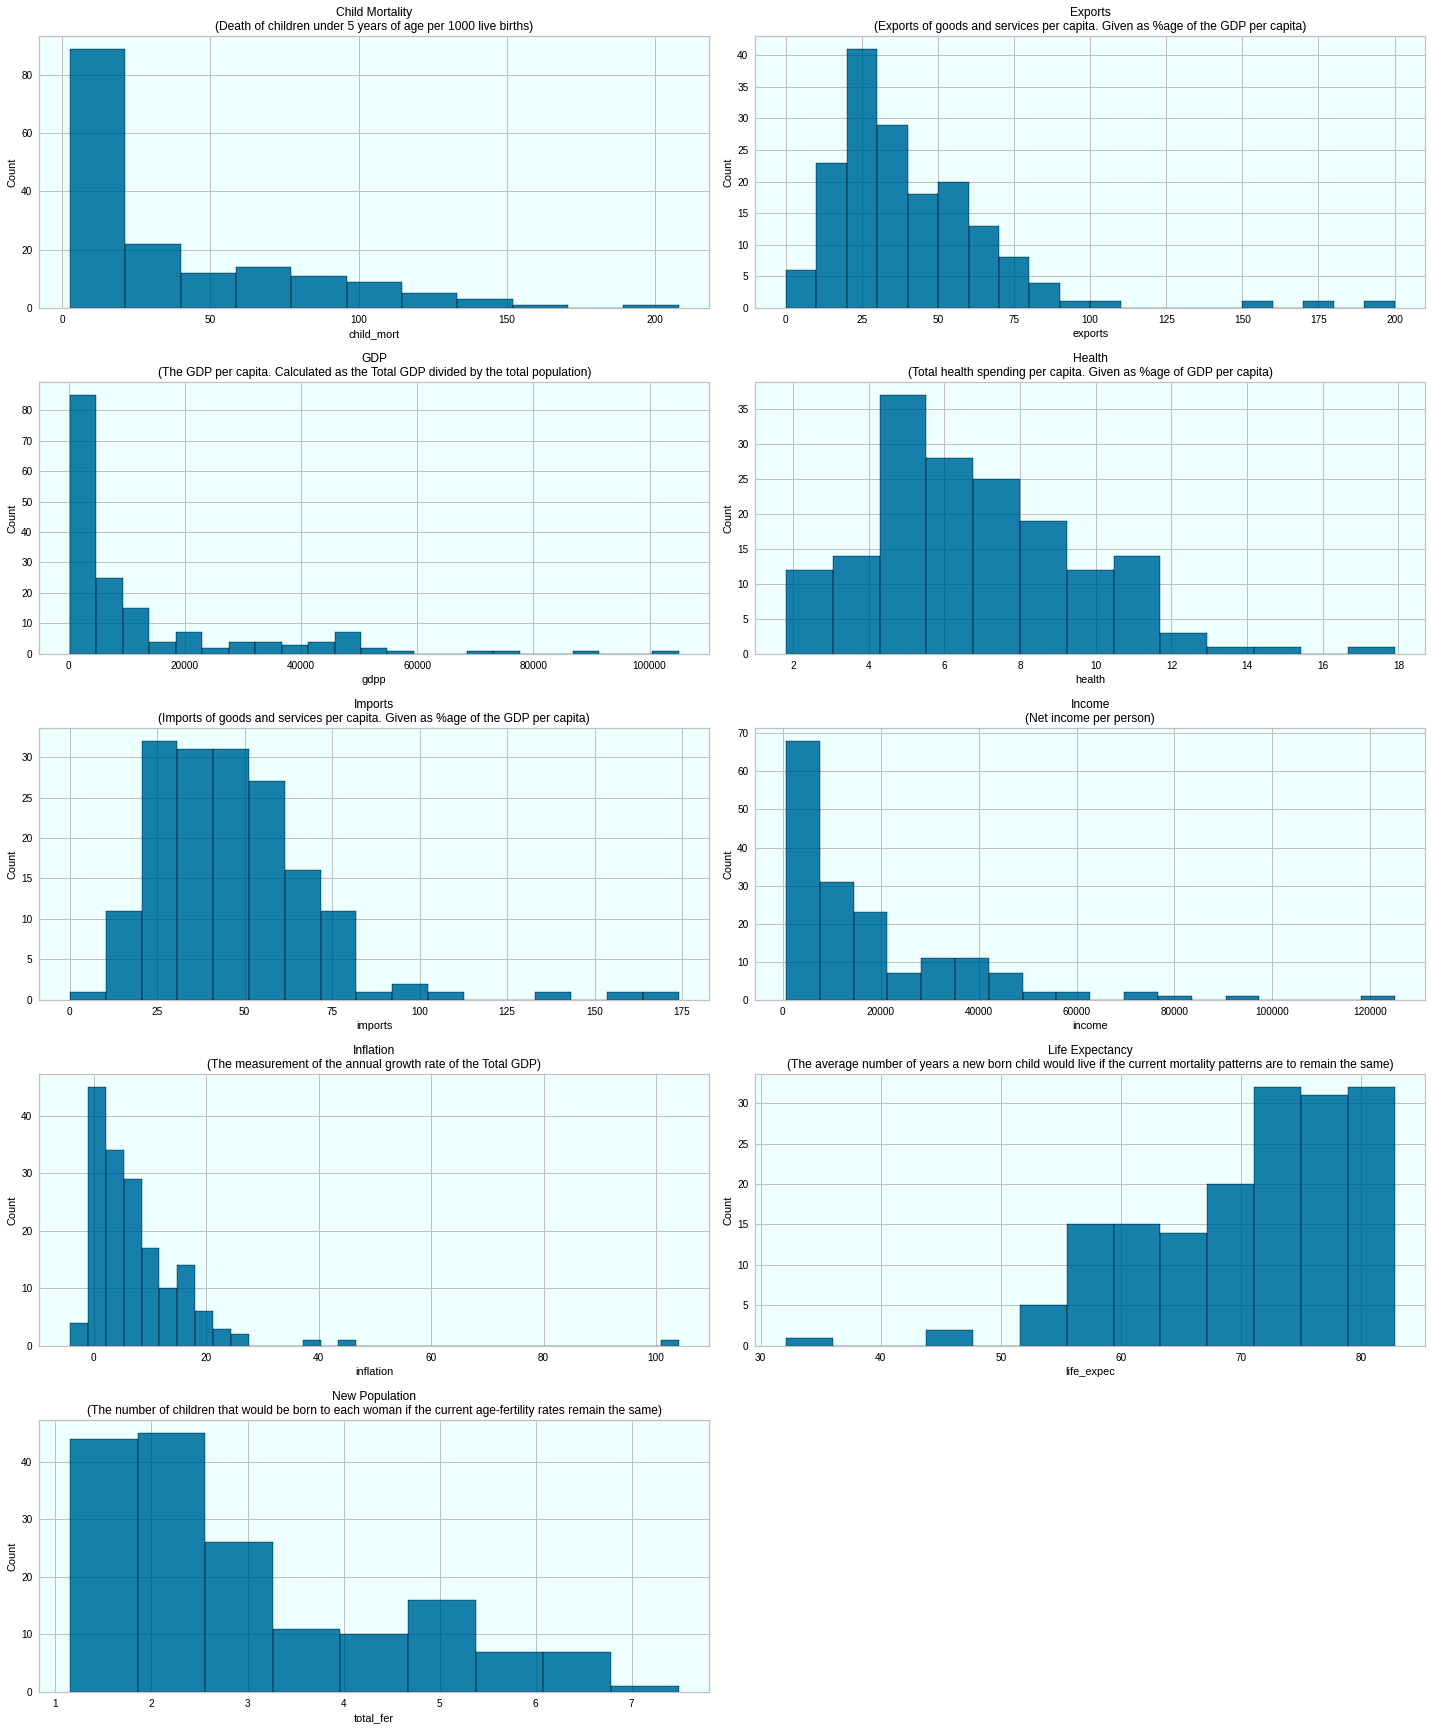
\includegraphics[width=\linewidth]{data-distribution}
    \caption{Data distribution of the country dataset}
    \label{fig:distribution}
\end{figure}

\subsection{Data Preparation}

Before running the data through machine learning algorithms, data preparation to construct and transform the data correctly is a necessary step to uncover insights or make predictions.

\subsubsection{Data Cleaning}

Data cleansing is necessary to feed the model with correct data. That’s why we’ve done all the cleansing on our datasets to ensure none of the columns have null values, inconsistent datatypes, or duplicate values so that no drop, conversion, or correction gets required later during the analysis, clustering, or modeling stages.

\subsubsection{Derived Metrics}

The variables export, health and imports are percentage values and hence wouldn't give a
clear picture of spending by the country. For example, two countries (Afghanistan, Albina) might have similar import percentages but do not necessarily have the same
GDP per capita. It doesn't give an accurate idea of which country is more developed than
the other. Hence we have deduced the imports, exports, and health spending value types
from percentage to actual values of their GDPP as shown in Table~\ref{tab:derived}.

\begin{table}[htp]
  \centering%
  \caption{Derived metrics\label{tab:derived}}
  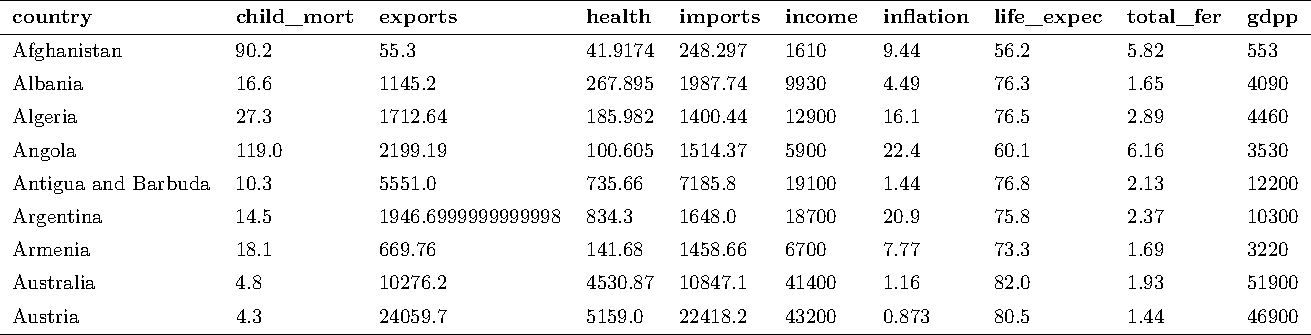
\includegraphics[width=\linewidth]{derived-metrics}
\end{table}

\subsubsection{Feature Scaling}

Feature scaling is vital for machine learning algorithms that calculate ranges between data since the distance of raw data values differs extensively. It helps make data points normalize so that the model can process them without any problems because the distance between them will be lower after the processing.

In our dataset, the features have incomparable units (metrics are percentages, dollar
values, and whole numbers), and the range values of the features also vary. So here, for
example, a change of 50 in one feature is quite significant, whereas in another it is
almost unnoticeable. This level of variance can negatively impact the performance of our
model, as this model is based on measuring distances, it can do this by giving more weight
to some features. And by using scaling methods, we can remove potential bias that the
model can have towards features with higher magnitudes. That's why we’ve eliminated the
column that contains the country information from our country dataset, as only numeric
values should be used in this case for our unsupervised learning-based model.

There are two common ways of rescaling. One is MinMax scaling, which subtracts the minimum
value in the feature and then divides it by the range as shown in Formula~\eqref{eq:minmax}.

\begin{equation}\label{eq:minmax}
X_{norm} = \frac{X - X_{min}}{X_{max}-X_{min}}
\end{equation}

The second is Standardization, where all features will be transformed to have the
properties of a standard normal distribution with mean \(=0\) and standard deviation
\(=1\) as seen in Formula~\eqref{eq:std}.

\begin{equation}\label{eq:std}
z = \frac{x - \mu}{\sigma}
\end{equation}

Where,
\begin{itemize}
\item[] Mean: \( \mu = \frac{1}{N} \sum_{i=1}^N (x_i)\)
\item[] Standard deviation: \(\sigma = \sqrt{\frac{1}{N} \sum_{i=1}^N (x_i - \mu)^2}\)
\end{itemize}


\begin{figure}[!htp]
    \centering
    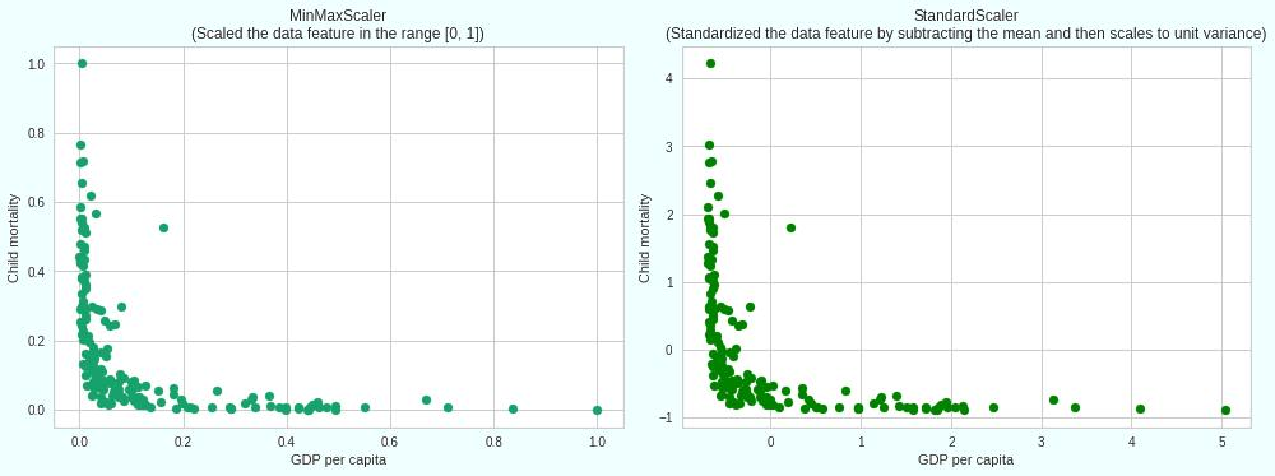
\includegraphics[width=\linewidth]{comparing-scaling-methods}
    \caption{Comparing the MinMax and Standard scaling methods}
    \label{fig:scaling}
\end{figure} 
In Figure~\ref{fig:scaling}, we've shown the comparison between the two scaling methods using features from the country dataset.

\subsection{Data Analytics}

\subsubsection{Uni-variate Analysis}

To choose the countries in the most urgent need of aid, we must identify and rank those
countries using the socio-economic and health factors. It'll help us to determine the
overall development of the country. Uni-variate analysis is the simplest way to do
that. Uni-variate analysis means that we're going to analyze the data involving only one
variable. This kind of analysis takes data, summarizes that data, and finds patterns in
data without dealing with causes or relationships. In Figure~\ref{fig:univariate}, we displayed the univariate analysis for our country dataset.

\begin{figure}[!htp]
  \centering 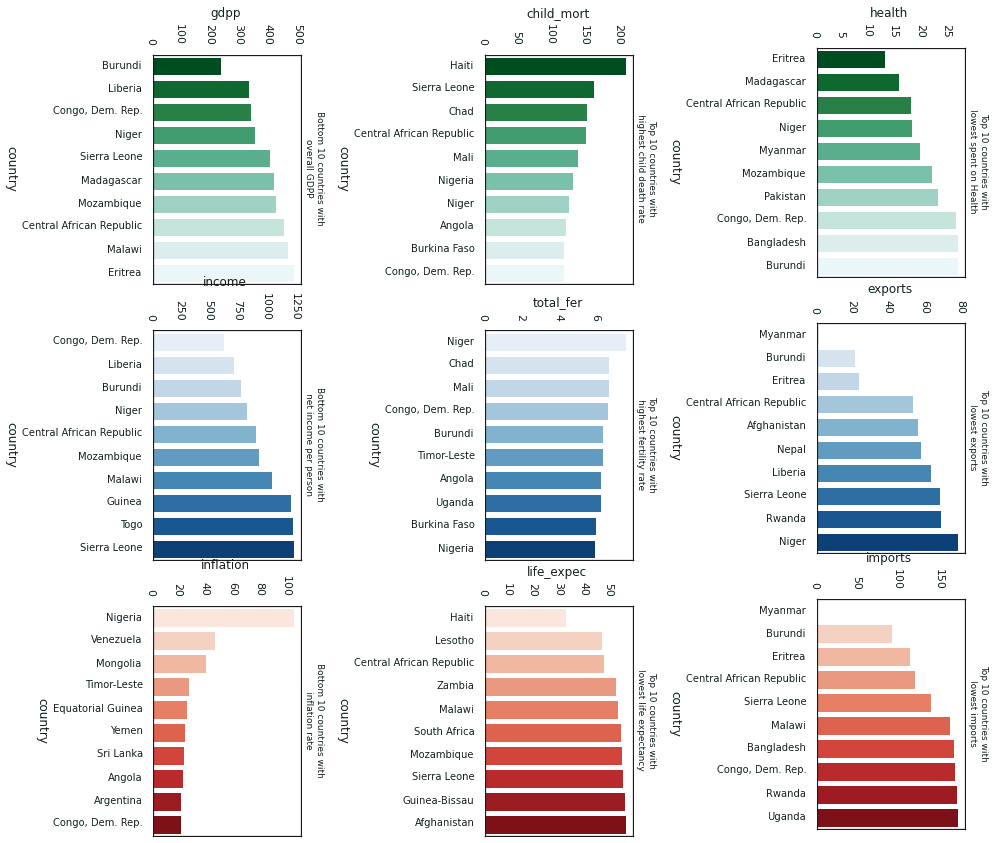
\includegraphics[width=11.5cm]{univariate-analysis}
  \caption{Uni-variate analysis of the country dataset}
  \label{fig:univariate}
\end{figure}
  

\subsubsection{Heatmap}

We've used heatmaps in this study to spot the magnitude of a phenomenon through the visual hue or intensity of color variation, giving a clear idea of how the phenomenon is clustered or varies over space. For example, finding the elementary correlation coefficients on our country dataset using a heatmap let us know which variables are significantly-correlated.

\begin{figure}[htp]
  \centering 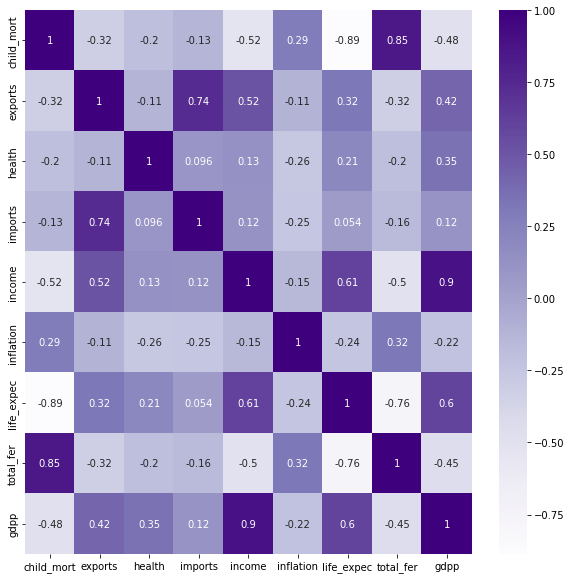
\includegraphics[width=11.5cm]{heatmap}
  \caption{Heatmap of the country dataset}
  \label{fig:heatmap}
\end{figure}
  
A linear correlation coefficient greater than zero indicates a positive relationship, whereas less than zero signifies a negative relationship. So, from the sample heatmap for the country dataset shown in Figure~\ref{fig:heatmap}, we can see the child mortality and life expectancy highly-correlated with a correlation of -0.89, child mortality and total fertility highly-correlated with a correlation of 0.85, imports and exports highly-correlated with a correlation of 0.99, life expectancy and total fertility highly-correlated with a correlation of -0.76.

\subsubsection{Pairplot}

We have used pair-plot visualizations for exploratory data analysis of our numeric columns present in experimental datasets to find the relationship between them where variables can be continuous or categorical. 

Pairplots create axes grids for sharing each numeric variable in our datasets across x, axes, and y-axes as columns and rows. It also helps visualize the subset of the variables and plots several types of variables on rows and columns.

\begin{figure}[!htp]
  \centering 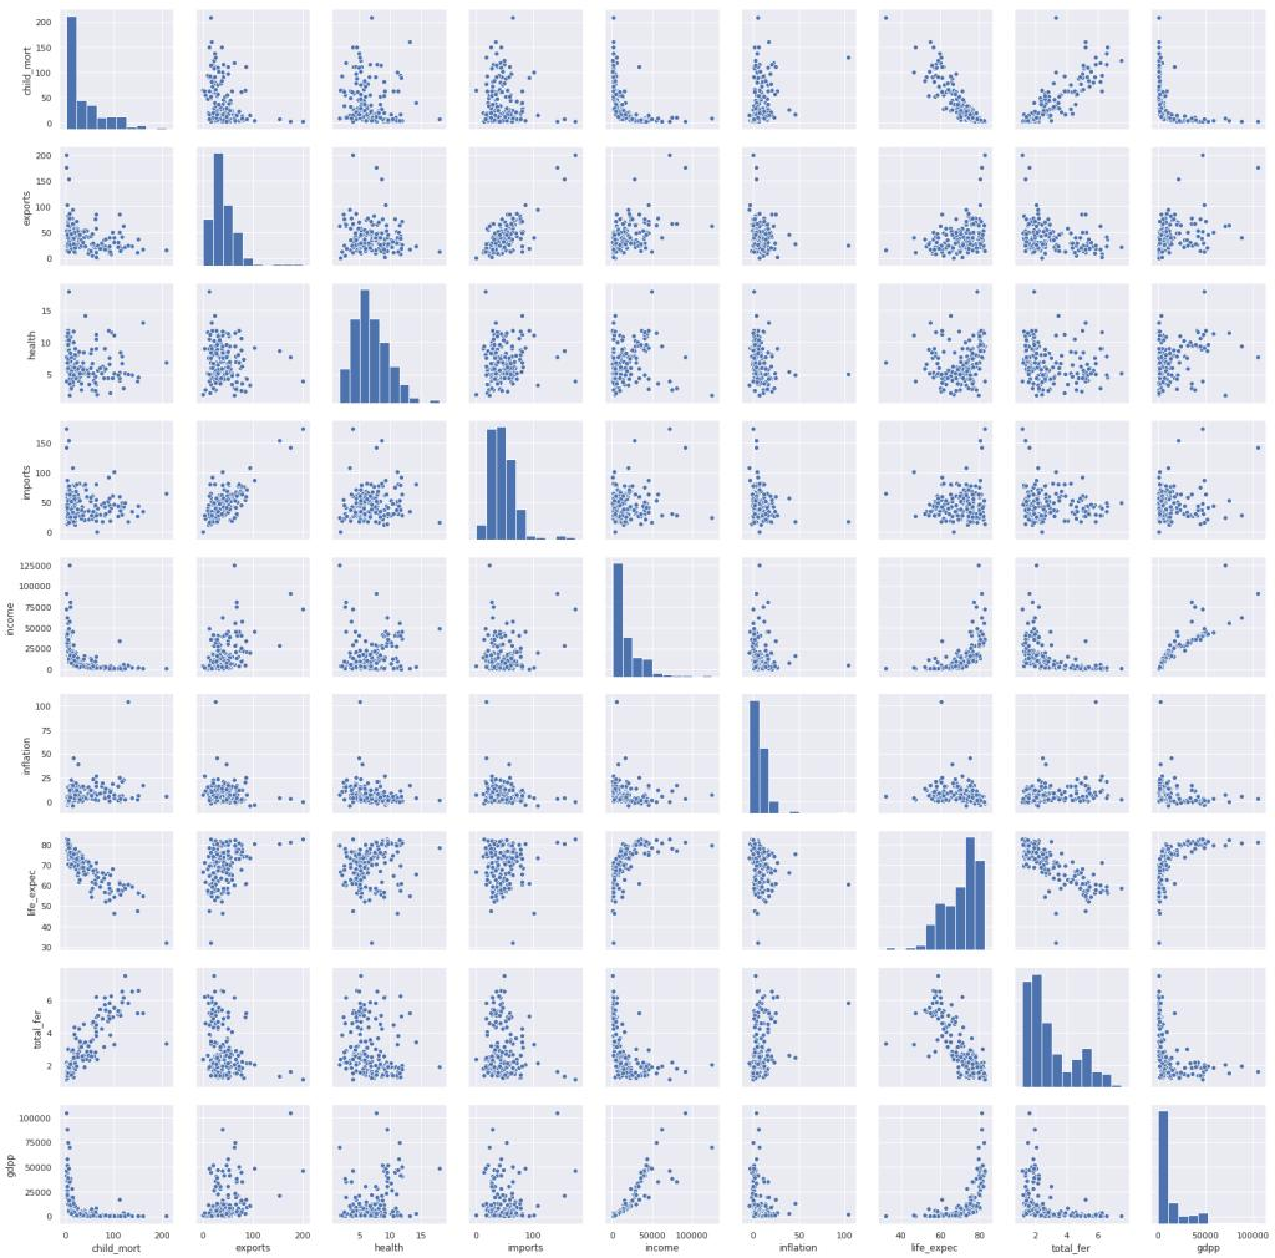
\includegraphics[width=.85\linewidth]{pairplot}
  \caption{Pairplot of the country dataset\label{fig:pairplot}}  
\end{figure}
  
As shown in Figure~\ref{fig:pairplot}, scatter plots show the pairwise relationships, and the distribution plots show the data distribution in the column. And through this visualization technique, we can confirm that many highly correlated variables exist in our datasets.

\section{Data Correlation Coefficients}
\label{sec:dcc}

During the exploratory analysis stage, we've used heatmaps (e.g. Figure~\ref{fig:heatmap})
to understand the attributes dependency in our existing datasets as the features may have
a positive, negative, or no relationship between them at all. Heatmaps are also necessary to
distinguish the appropriate type of correlation coefficient before deciding whether to
keep the variable in the dataset or not for later analysis and modeling steps. Generally,
four types of correlations get used during the statistical study. Pearson correlation,
Kendall rank correlation, Spearman correlation, and the Point-Biserial correlation. But
Point-biserial correlation is only handy when measuring the strength and direction of the
association between one continuous variable and one dichotomous variable. So, below we've
used the other three to confirm the associations between variables. And after looking at
the results, we found some features considered for elimination due to high
correlation. For example, life expectancy, due to high correlation with child mortality;
total fertility, due to high correlation with child mortality; income, due to high
correlation with GDPP.

\subsection{Pearson Correlation}

The Pearson correlation coefficient is a popular and widely used measure to test linear
relationships between two normally distributed continuous variables. The covariance method
Pearson correlation uses makes it one of the best options for calculating the relationship
between variables of interest. The formula for the Pearson correlation coefficient is:

\[
  r = \frac{{}\sum_{i=1}^{n} (x_i - \overline{x})(y_i - \overline{y})}
  {\sqrt{\sum_{i=1}^{n} (x_i - \overline{x})^2(y_i - \overline{y})^2}}
\]
Where,
\begin{itemize}[itemsep=-1.5ex]
\item[\(r\):] correlation coefficient
\item[\(x_{i}\):] values of the x-variable in a sample
\item[\(\bar{x}\):] mean of the values of the x-variable
\item[\(y_{i}\):] values of the y-variable in a sample
\item[\(\bar{y}\):] mean of the values of the y-variable
\end{itemize}
But when the Pearson correlation is applied to a population, the formula is: 

\[
  \rho = \frac{\text{cov}(X,Y)}{\sigma_x \sigma_y}
\]
Where,
\begin{itemize}[itemsep=-1.5ex]
\item[\(\rho\):] the population Pearson correlation coefficient
\item[\(cov\):] the covariance
\item[\(\sigma_X\):] the standard deviation of \(X\)
\item[\(\sigma_Y\):] the standard deviation of \(Y\)
\end{itemize}

\begin{figure}[!htp]
  \centering 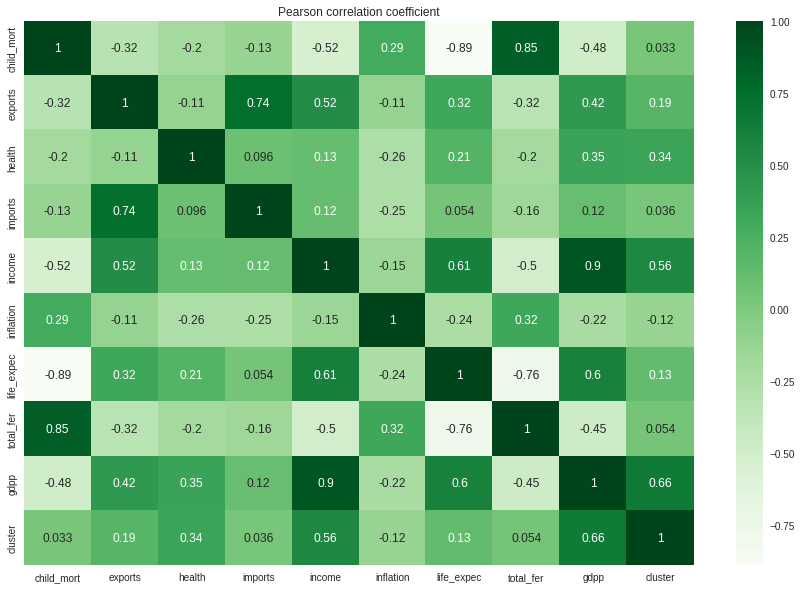
\includegraphics[width=.9\linewidth]{pearson}
  \caption{Pearson correlation of the country dataset}
  \label{fig:pearson}
\end{figure}

In Figure~\ref{fig:pearson}, a heatmap of Pearson correlation for our country dataset is shown.  Generally, in the Pearson coefficient, the value of 1 represents a perfectly
positive, -1 is a perfect negative, and 0 indicates the absence of a relationship between
variables.

\subsection{Kendall Correlation}

Kendall rank correlation coefficient, widely known as Kendall’s Tau coefficient, is the best alternative to the Pearson and Spearman correlation coefficient.

\begin{figure}[!htp]
  \centering 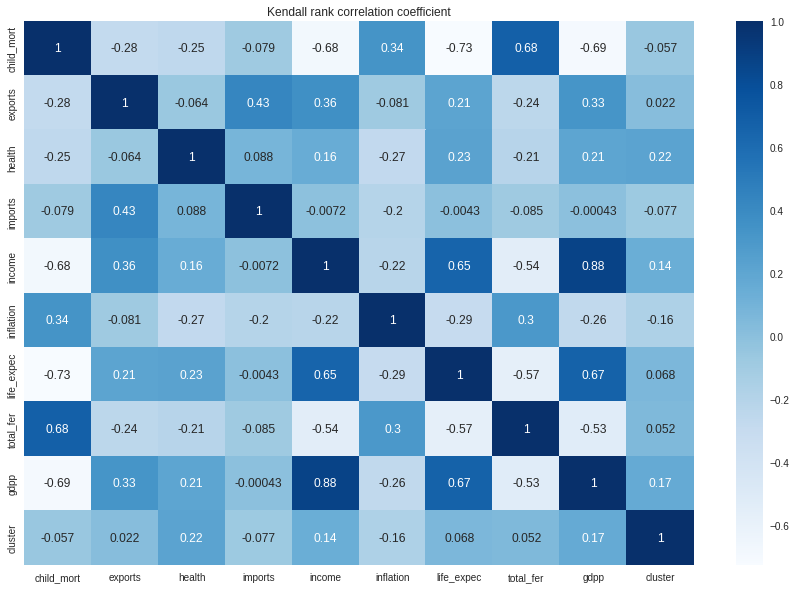
\includegraphics[width=\linewidth]{kendall}
  \caption{Kendall's Tau correlation of the country dataset\label{fig:kendall}}  
\end{figure}
  
Because it measures the degree of a monotone relationship between variables like the Pearson coefficient and calculates the dependence between ranked variables like Spearman. But other correlation coefficients use the observations as the basis of the correlation, but Kendall’s correlation coefficient is different. It takes a pair or set of observations, known as the sample, and then determines the strength of association between the pairs based on the pattern of concordance and discordance. The formula for the Kendall's Tau is:

\[
  \tau = \frac{c-d}{c+d} = \frac{S}{
	\left(
      \begin{matrix}
        n \\
        2
      \end{matrix}
    \right)}
  = \frac{2S}{n(n-1)}    
\]
Where,
\begin{itemize}[itemsep=-1.5ex]
\item[\(c:\)] the number of concordant pairs
\item[\(d:\)] the number of discordant pairs
\end{itemize}

But if the ties are present among the two ranked variables, then the following equation is used instead:

\[
  \tau = \frac{S}{\sqrt{n(n-1)/2-T}\sqrt{n(n-1)/2-U}}
\]
Where,
\begin{itemize}[itemsep=-1.5ex]
\item[\(t:\)] number of observations of variable x that are tied
\item[\(u:\)] number of observations of variable y that are tied
\item[] \(T = \sum_t t(t-1)/2\)
\item[] \(U = \sum_u u(u-1)/2\)
\end{itemize} 
In Figure~\ref{fig:kendall}, a heatmap of Kendall's Tau correlation for our country dataset is shown.
\subsection{Spearman Correlation}

Spearman’s correlation is similar to the Pearson correlation coefficient because it measures the relationship between two variables on the ranked data. But unlike Pearson, Spearman's correlation is not limited to continuous data only, as it also works for ordinal attributes.

\begin{figure}[htp]
    \centering
    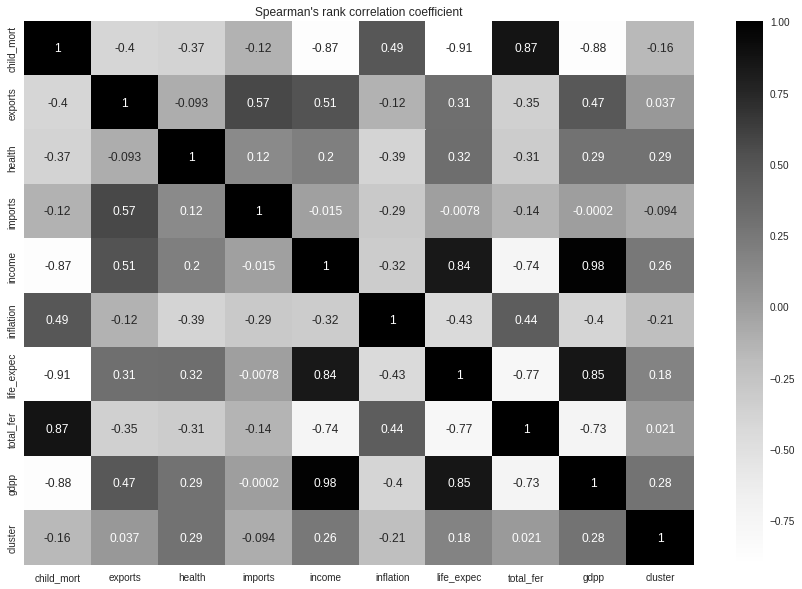
\includegraphics[width=.9\linewidth]{spearman}
    \caption{Spearman's correlation of the country dataset}
    \label{fig:spearman}
\end{figure}

So ρ will always be a value within -1, 1 and will correspond to the direction of the relationship. If the value of rho goes far from zero, then the relationship between the two variables will get stronger. The formula for the Spearman's correlation is:

\[
  \rho = 1- {\frac {6 \sum d_i^2}{n(n^2 - 1)}}
\]
Where,
\begin{itemize}[itemsep=-1.5ex]
\item[\(\rho\):] Spearman's rank correlation coefficient
\item[\(d\):] the pairwise distances of the ranks of the variables \(x_i\) and \(y_i\)
\item[\(n\):] the number of samples
\end{itemize}
In Figure~\ref{fig:spearman}, a heatmap of Spearman correlation for our country dataset is shown.
\section{Principal Component Analysis (PCA) Application}

Principal Component Analysis (PCA) is a technique used to identify a smaller number of
uncorrelated variables from big datasets to simplify the complexity in high-dimensional
data while retaining the patterns and trends.  It reduces the dimensionality of a data set
while keeping approximately most of the possible variations present there. PCA does it via
transforming to a new set of variables, the principal components (PCs), which are
uncorrelated, and ordered so that the first few retain most of the variation present in
all of the original variables.

We have used PCA (Figure~\ref{fig:pca}) in our study because we need to remove the redundancies in the data and
find the most important directories where the data is aligned. It will help visualize
complex data sets, improve our model performance, and many more.

\subsection{PCA with Scaled Data}

\begin{figure}[!htp]
  \centering
  \subcaptionbox{PCA with StandardScaler\label{fig:standard-pca}}{%
    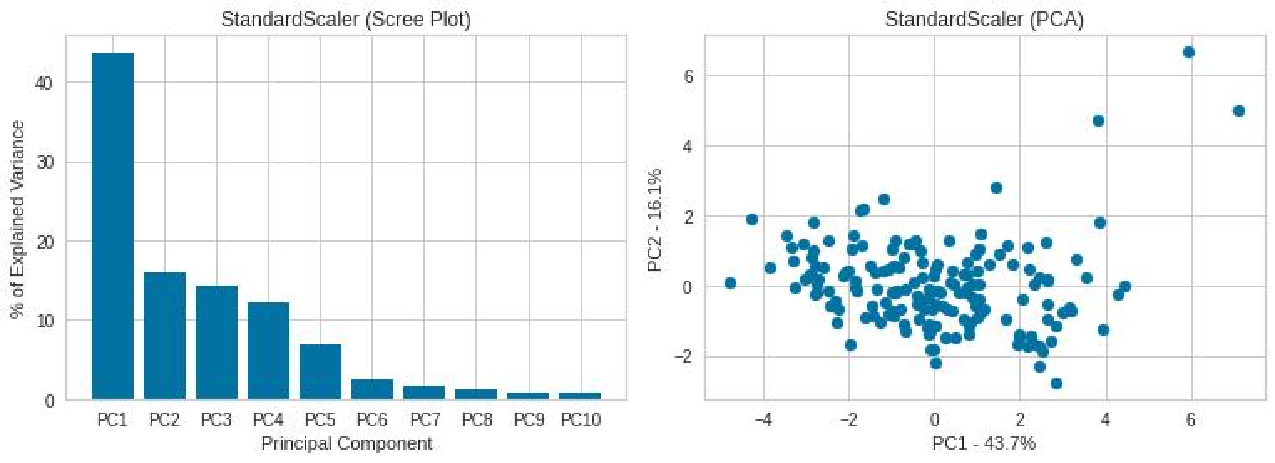
\includegraphics[width=\linewidth]{standard-scaler}}\\\bigskip
  \subcaptionbox{PCA with MinMaxScaler\label{fig:minmax-pca}}{%
    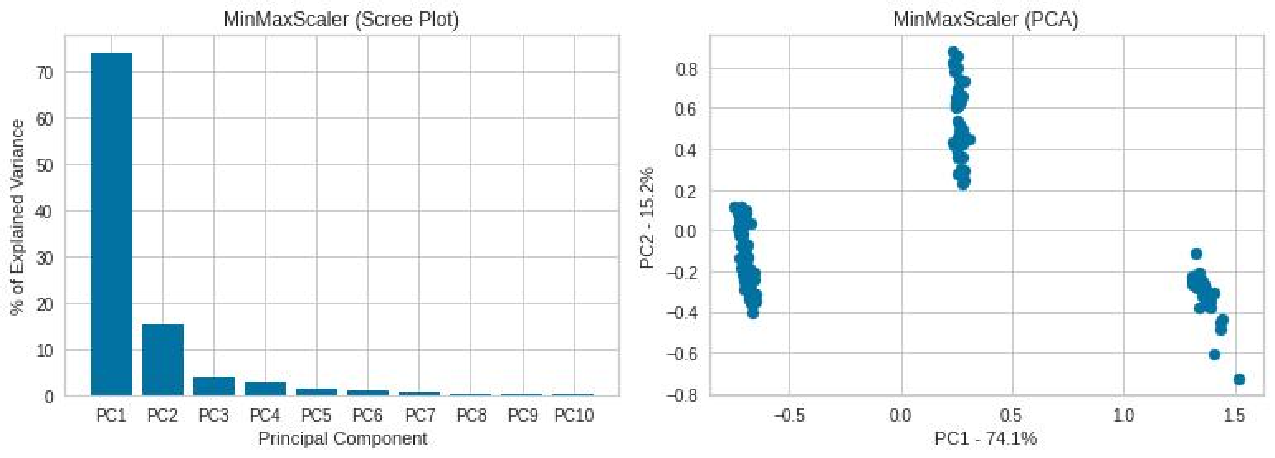
\includegraphics[width=\linewidth]{minmax-scaler}}
  \caption{Principal Component Analysis\label{fig:pca}}
\end{figure}

From the PCA shown in figures \ref{fig:standard-pca} and \ref{fig:minmax-pca}, we can see both the standardized and normalized versions of the original dataset have four principal components that can explain about 90\% of the distribution of the original dataset.

\section{Hopkins Statistics Test}

The Hopkins statistic is a way of measuring the clustering tendency of a data set. Hopkins
scores that are close to 1 tends to indicate the data is highly clustered, values around
0.5 mean random data, and 0 mean uniformly distributed data. The Hopkins statistic is
calculated as \(1-H\).

\[
    H=\frac{\sum_{i=1}^m{u_i^d}}{\sum_{i=1}^m{u_i^d}+\sum_{i=1}^m{w_i^d}}
\]
Where,
\begin{itemize}[itemsep=-1.5ex]
\item[\(u_i\):] nearest neighbour distances from uniformly generated sample points to
  sample data
\item[\(w_i\):] nearest neighbour distances within sample data
\end{itemize}
In our case, we calculated the Hopkins score to verify whether the data is OK for clustering or not. And found a score of 0.83, which is a good score for clustering.

\section{Model Building}
\label{sec:mod}

We can now begin to build unsupervised learning models as we do not want any external impact or standard to judge the model's classification performance. Data modeling is the process of analyzing data types and producing a descriptive diagram of the relationship between different types of information to help classify data into structures that can be easily understood and used. We've worked on an unsupervised method called clustering. Clustering can automatically discover natural groupings in data, making it unique from predictable models for not having a target value. That's why in clustering, the process outcome can't get guided by a known result. There are no right or wrong answers for these models as the value is only determined by the model's ability to obtain interesting patterns in data to partition the data into some group of logical groupings with useful descriptions.

\subsection{K-means Clustering}

K-means clustering is an unsupervised learning algorithm that we used for being the
fastest and most efficient algorithm to group the unlabeled (without defined categories or
groups) dataset into different clusters even when very little information is available
about data.

K-means finds the best centroids by oscillating between 
\begin{enumerate}
\item selecting data points to clusters based on feature similarity
\item choosing the points at the center of a cluster based on the prevailing assignment of
  data points to clusters
\end{enumerate}
    
The k-means algorithm partitions a given set of observations into a predefined amount of $k$ clusters. It starts with a random set of $k$ center-points ($\mu$). Then during each update step, all observations $x$ are assigned to their nearest center-point (Equation~\ref{eqn:kmeans_assign_step}). In the standard algorithm, only one assignment to one center is possible. If multiple centers have the same distance to the observation, a random one gets chosen.

\begin{equation}
S_i^{(t)} = \big \{ x_p : \big \| x_p - \mu^{(t)}_i \big \|^2 \le \big \| x_p - \mu^{(t)}_j \big \|^2 \ \forall j, 1 \le j \le k \big\}
\label{eqn:kmeans_assign_step}
\end{equation}
Afterward, the center points get repositioned by computing the mean of the assigned observations to the respective center points (Equation~\ref{eqn:kmeans_update_step}).

\begin{equation}
\mu^{(t+1)}_i = \frac{1}{|S^{(t)}_i|} \sum_{x_j \in S^{(t)}_i} x_j
\label{eqn:kmeans_update_step}
\end{equation}
The update process keeps occurring until all observations remain at the assigned
center points, and therefore the center points would not be updated anymore.

This suggests that the k-means algorithm tries to optimize the objective function (Equation~\ref{eqn:kmeans_objective_function}). As there is only a finite number of possible assignments for the number of centroids and observations available and each iteration has to result in a better solution, the algorithm always ends in a local minimum.

\begin{equation}\label{eqn:kmeans_objective_function}
J = \sum_{n=1}^{N} \sum_{k=1}^{K} r_{nk} ||x_n - \mu_k||^2
\end{equation}
\hspace{13.2em}with
\vspace*{-3ex}
\[
  r_{nk} = \begin{cases}
    % 1 & \text{if } k = \arg \min_j ||x_n - \mu_j||^2 \\
    1 & x_n \in S_k \\
    0 & \text{otherwise}
  \end{cases}
\]

After running the K-means model with different versions of the dataset (normalized and standardized dataset, and a PCA with four components), we discerned that the optimal number of clusters is still 3 with different levels of inertia.

\subsection{Optimal Numbers of Clusters}

Another fundamental step for any unsupervised algorithm such as k-means clustering (the user needs to specify the number of clusters K that needs generating) is determining the optimal cluster number into which the data may get clustered. The optimal number of K clusters is the one that maximizes the average silhouette over a range of possible values for K.

\subsubsection{Elbow Method}

The Elbow Method is one of the most popular methods to determine this optimal value of K. The elbow method runs k-means clustering on the dataset for a range of values for K and then computes the clustering algorithm for different values of K for all clusters.

\begin{figure}[!htp]
  \centering 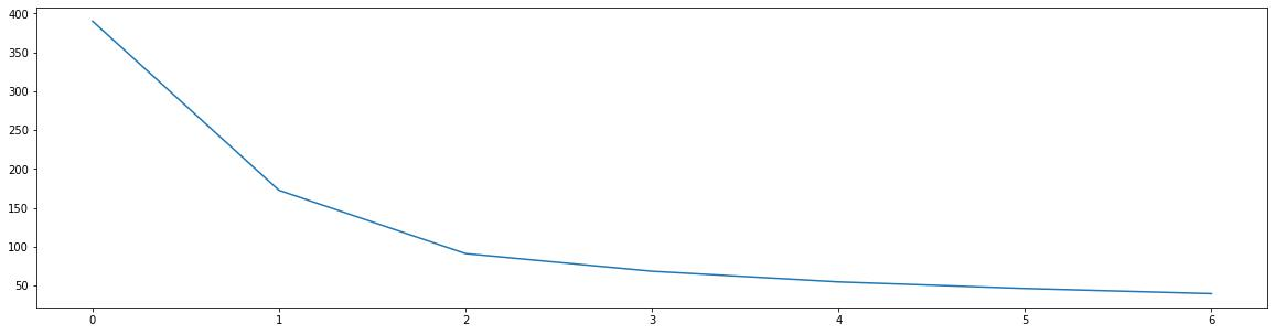
\includegraphics[width=\linewidth]{elbow-method}
  \caption{Elbow method\label{fig:elbow}}  
\end{figure}
  
In our case, the elbow curve shown in Figure~\ref{fig:elbow} confirms that we're good to proceed with either 4 or 5 clusters.

\subsubsection{Silhouette Analysis}

Silhouette analysis interprets and validates consistency within clusters of data by measuring the quality of clustering through discovering how well each object lies within it. A high average silhouette width indicates a good clustering (the silhouette score ranges from -1 to 1).

\[
    \text{silhouette score}=\frac{p-q}{max(p,q)}
\]
Where,
\begin{itemize}[itemsep=-1.5ex]
\item[\(p\):] mean distance to the points in the nearest cluster
\item[\(q\):] mean intra-cluster distance to all the points
\end{itemize}

The silhouette method helped us complement all our further cluster analysis stages. It corrected our study by showing scores close to 0, an indication that clusters are overlapping. And an increase in clusters later showed negative values in the scale, which means that clusters might have samples that have been assigned to the wrong cluster.

\begin{figure}[!htp]
    \centering
    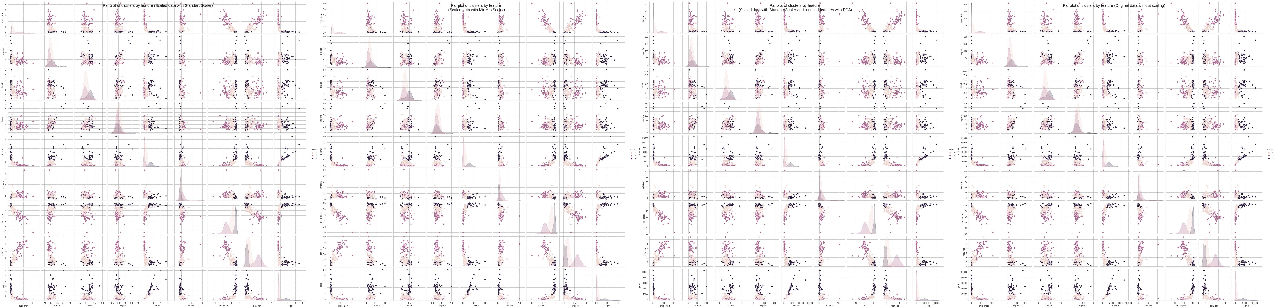
\includegraphics[width=\linewidth]{cluster-analysis}
    \caption{Pairplot of clusters by feature\label{fig:cluster-analysis}}    
\end{figure}

After finding out the silhouette score, we ran the model with our two types of scaled datasets (StandardScaler, MinMaxScaler) and using PCA as shown in the pairplot of Figure~\ref{fig:cluster-analysis}, we confirmed the overlapping between clusters. We saw that cluster 2 is more spread out, and clusters 0 and 1 tends to overlap. 

\subsection{Hierarchical Clustering}

We've used hierarchical clustering to group the unlabeled data points having similar characteristics. Because as mentioned earlier, K-means clustering is a division of the set of data objects into non-overlapping subsets or clusters where each data object is in exactly one subset. On the other hand, hierarchical clustering is an unsupervised clustering algorithm that'll let us have a set of nested clusters arranged as a tree with a predetermined ordering from top-to-bottom allowing us to build tree structures from data similarities.

But in hierarchical clustering, clusters or subsets are blended based on the length or distance between them, and to calculate the distance between the clusters, we can use the single and complete linkage clustering.

\begin{figure}[htp]
  \centering%
  \subcaptionbox{Distance in single linkage\label{fig:single}}{%
    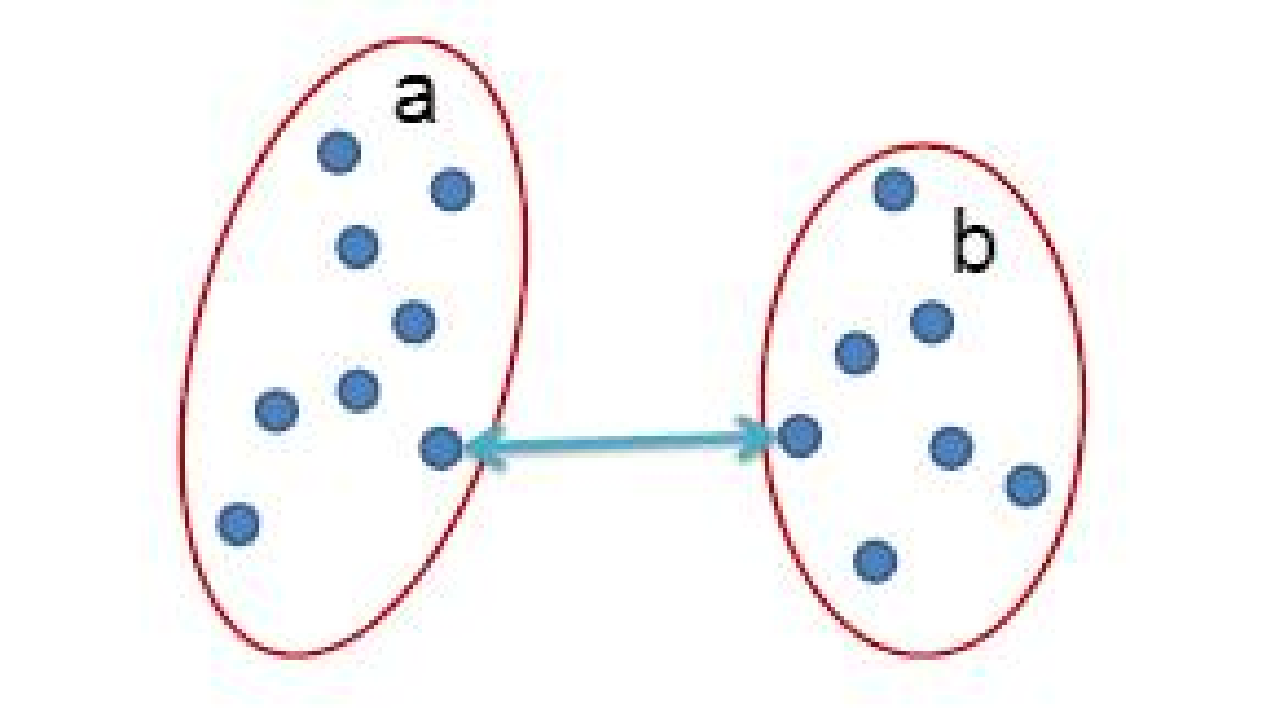
\includegraphics[width=.4\linewidth]{single}}\qquad\qquad
  \subcaptionbox{Distance in complete linkage\label{fig:complete}}{%
    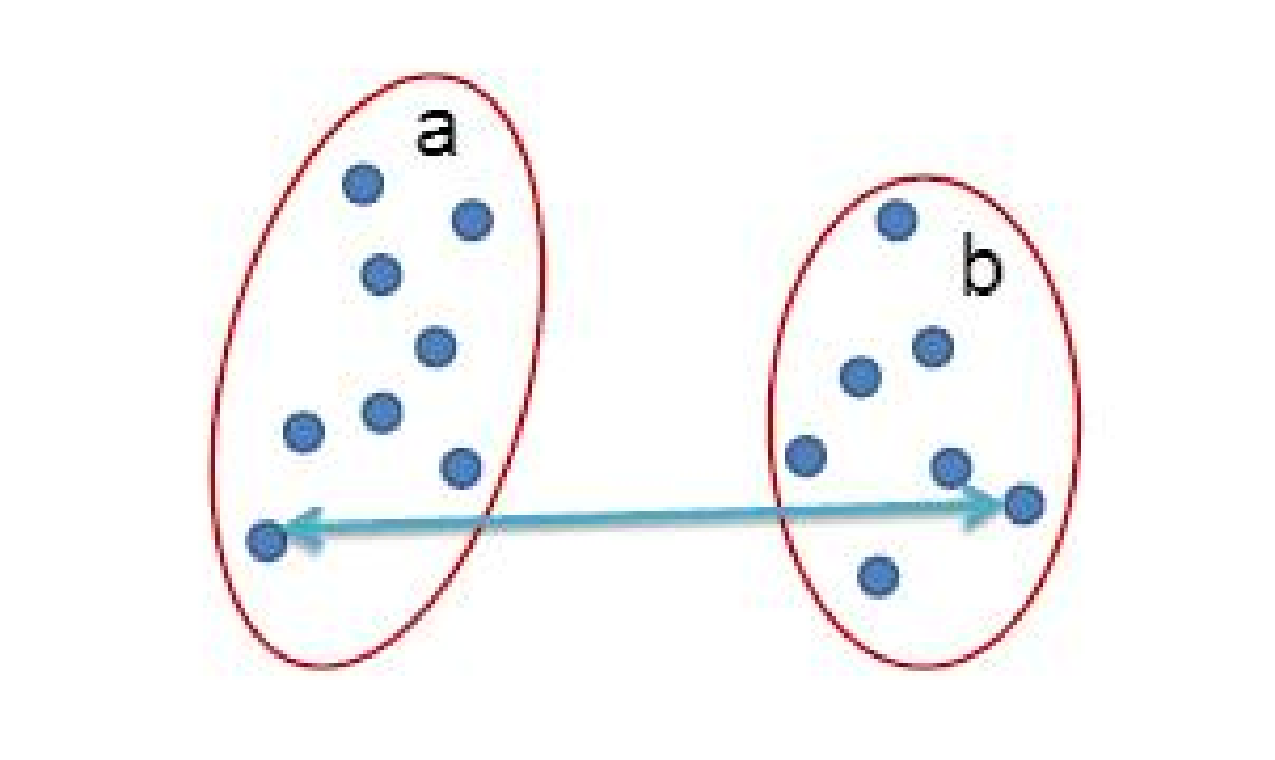
\includegraphics[width=.4\linewidth]{complete}}
  \caption{Hierarchical clustering\label{fig:hier-clustering}}
\end{figure}

\subsubsection{Single Linkage}

In single linkage hierarchical clustering, the distance between the two clusters is
explained as the shortest or minimum distance between members of the two clusters.
For instance, the distance between clusters ``a'' and ``b'' shown in Figure~\ref{fig:single}
in single linkage is equal to the length of the arrow between their two closest points,
\(L(a,b) = min(D(x_{ai},x_{bj})\). In Figure~\ref{fig:single-linkage}, we can see the single linkage clustering output for our dataset in a dendrogram. 

\begin{figure}[htp]
  \centering 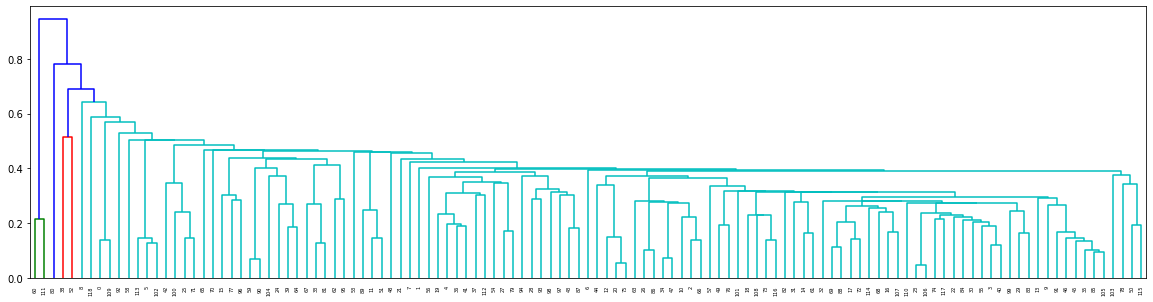
\includegraphics[width=.9\linewidth]{single-linkage}
  \caption{Single linkage clustering output}
  \label{fig:single-linkage}
\end{figure}
  
\subsubsection{Complete Linkage}

In complete linkage hierarchical clustering, the distance between two clusters is interpreted as the longest or maximum distance between members of the two clusters.  
Like, the distance between clusters ``a'' and ``b'' shown in Figure~\ref{fig:complete} is
equal to the length of the arrow between their two furthest points,
\(L(a,b) = max(D(x_{ai},x_{bj})\). In Figure~\ref{fig:complete-linkage}, we can see the complete linkage clustering output for our dataset in a dendrogram. 

\begin{figure}[htp]
  \centering 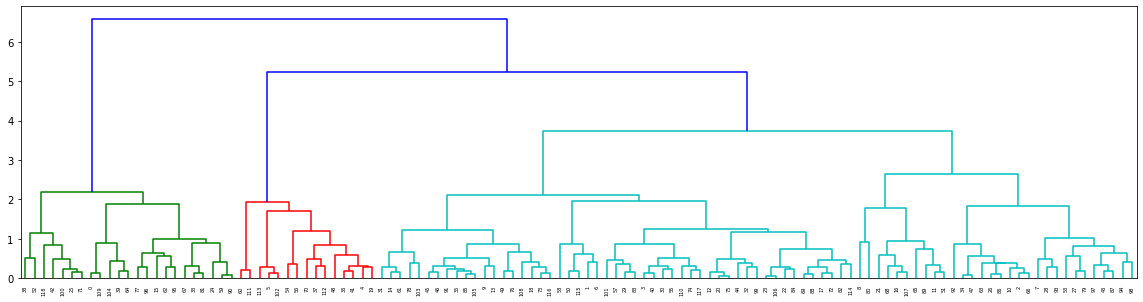
\includegraphics[width=.9\linewidth]{complete-linkage}
  \caption{Complete linkage clustering output}
  \label{fig:complete-linkage}
\end{figure}

\subsection{Cluster Characteristics}

\subsubsection{Cluster Descriptions}

Before moving to the final analysis, we've finalized our clusters. The first one is Cluster 0, which holds the average values for all features compared to the other two. The second one is Cluster 1. It has the most negative values out of all. And finally, the third one, Cluster 2, has the most firm or positive values of all features.

\subsubsection{Clusters Location in the World}

To visualize the regions our three clusters are covering, we've used geospatial plotting shown in Figure~\ref{fig:location}. Geospatial data visualization helps integrate interactive visualization into traditional maps.

\begin{figure}[htp]
    \centering
    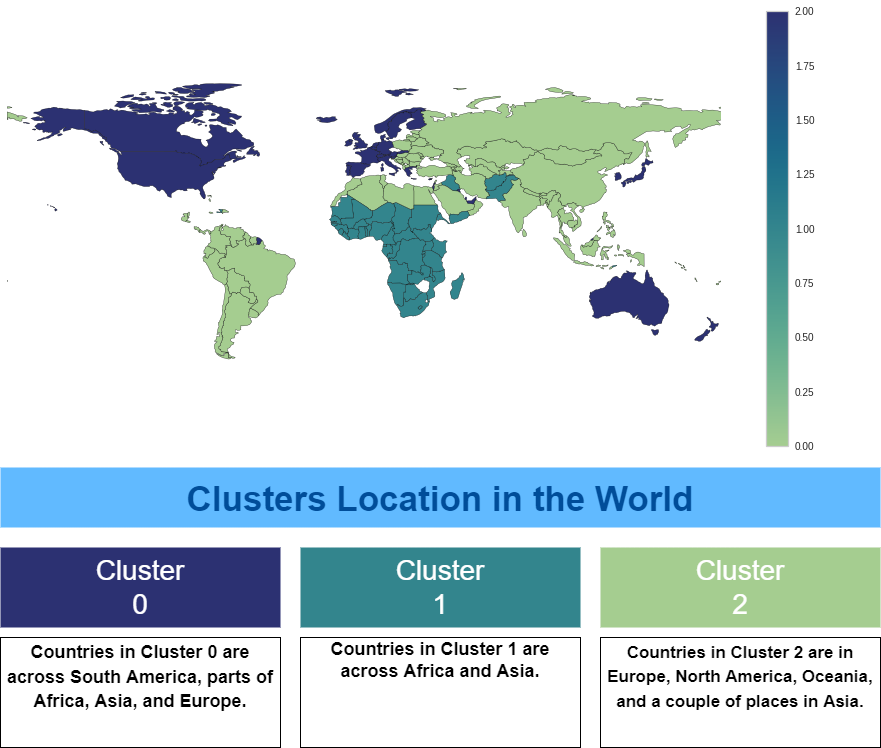
\includegraphics[width=.7\linewidth]{clusters-location}
    \caption{Clusters location in the world}
    \label{fig:location}
\end{figure}

\section{Final Analysis}

After the initial assessments, at the time, when we plotted the clusters and looked at the graphs, we observed clusters being overlapped and spread out. Applying PCA as an alternative did not make much difference either. Though we were able to identify certain patterns in the data and group the countries into three clusters. But still, we should not depend entirely on this result to recommend countries that should receive aid funding. There are a few other ways to explore before making this recommendation. Because to this point, our study only confirmed a general understanding of intuition on this topic. The clustering we've done so far is a preliminary preprocessing step, and further analysis is needed.
  
So to begin, at first, we've dropped the features with high correlation as pointed out in the Data Correlation Coefficients section (Section~\ref{sec:dcc}). Features identified as having high correlation earlier in this chapter have resulted in two clusters with high inertia (see Figure~\ref{fig:sse}).

\begin{figure}[!htp]
  \centering 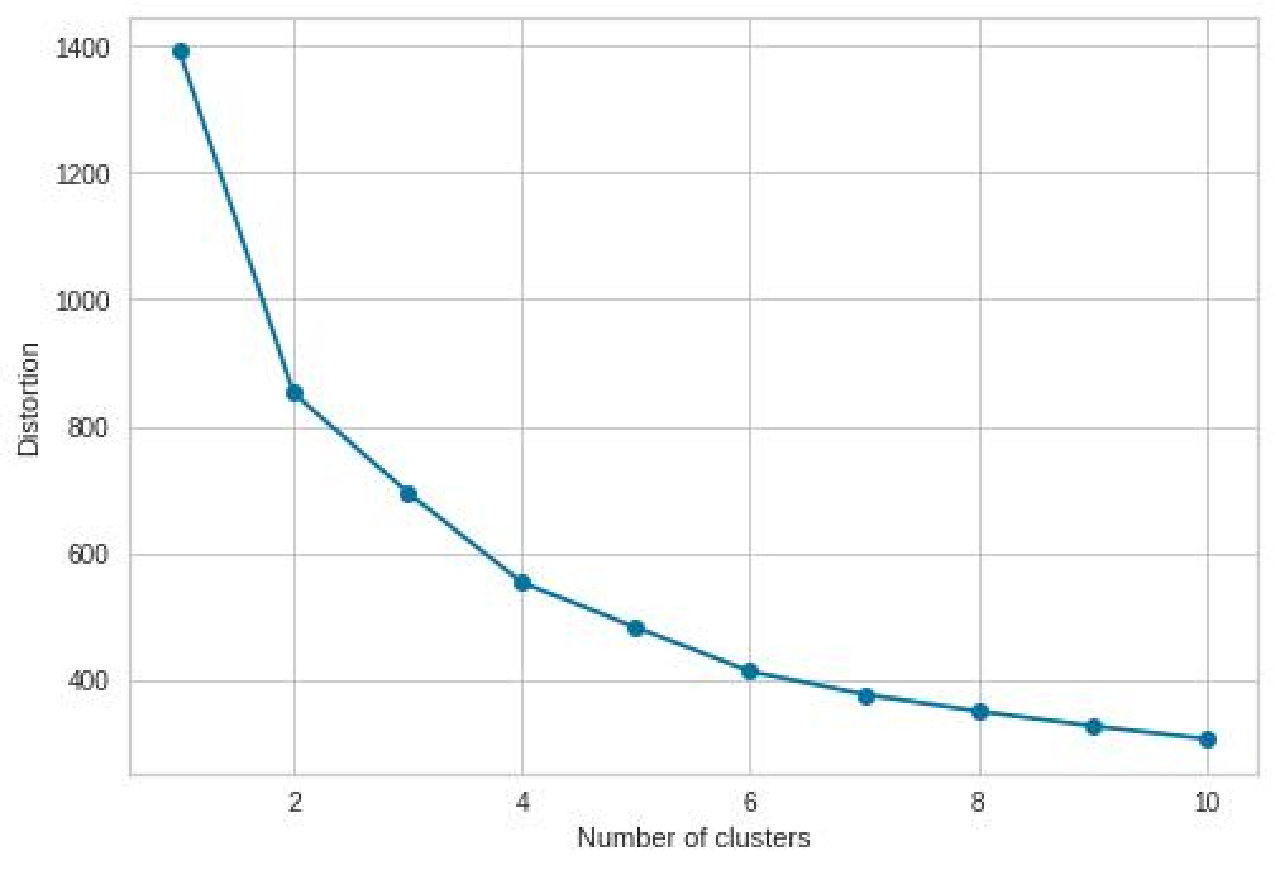
\includegraphics[width=.75\linewidth]{sse}
  \caption{Cluster intertia\label{fig:sse}}  
\end{figure}

Next, we focused on cluster 2, which has the most strong values of all features, to further explore the formation of this cluster and tried to see if any countries from here should be in the final aid recommendation.

\begin{figure}[!htp]
  \centering 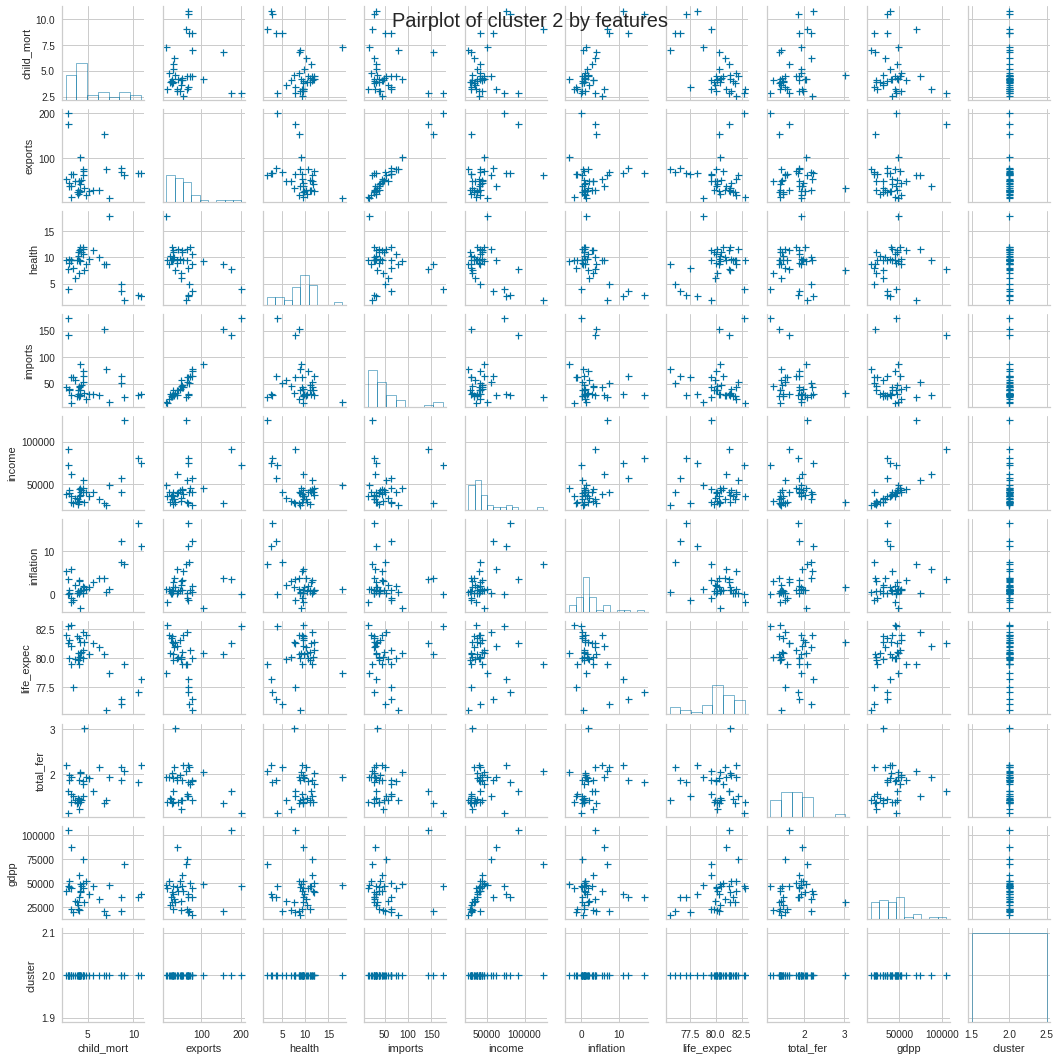
\includegraphics[width=.8\linewidth]{cluster2}
  \caption{Pairplot with Cluster 2 features\label{fig:cluster2}}
\end{figure}

From the pair plot of cluster 2 by features, as shown in Figure~\ref{fig:cluster2}, we can notice that the outliers found in the features of cluster 2 are generally more positive and distant from values from clusters 0 and 1. So, it's clear that countries in this cluster will not get aid fundings.

We've also found some clusters with high overlapping, and we need to investigate further to answer the question at hand with more aiding data. And to do this, we'll now consolidate a new feature called MPI from OPHI's Multidimensional Poverty Index dataset. The MPI will act as the Dependent Variable (DV), and the data we already have been working on will be the Independent Variables (IV). Here, the Independent Variable (IV) is a variable that is adjusted to see how it changes something else where the dependent variable (DV) is the one getting measured. Simply we can think of IV as the cause and DV as the effect. We'll use Multiple Linear Regression as a way to quantify the relationship between several IVs and a DV.

\begin{figure}[!htp]
    \centering
    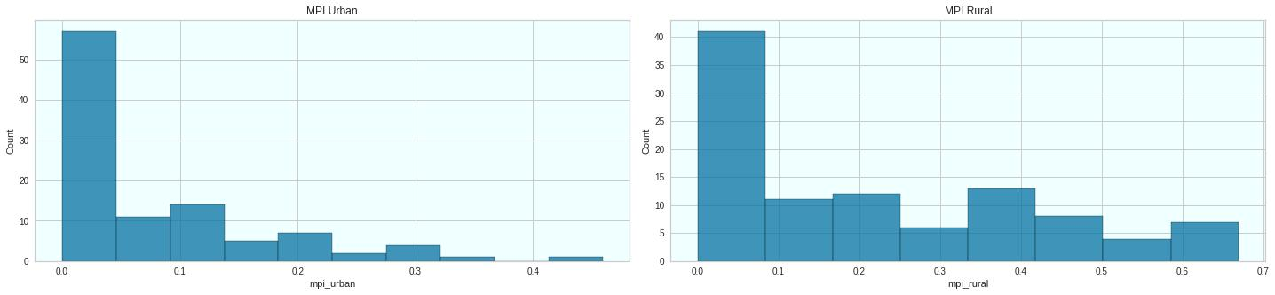
\includegraphics[width=\linewidth]{mpi-urban-rural}
    \caption{MPI urban and rural histplot}
    \label{fig:mpi-urban-rural}
\end{figure}

For this analysis, we will focus on MPI Urban and MPI Rural. It's because the MPI measure reflects both the incidence and intensity of poverty. Here, the percentage of the poor population is the incidence. And the rate of deprivations suffered by each person or household on average is the intensity of poverty. In Figure~\ref{fig:mpi-urban-rural}, the histplot of these two newly added features are shown. 

\begin{figure}[!htp]
    \centering 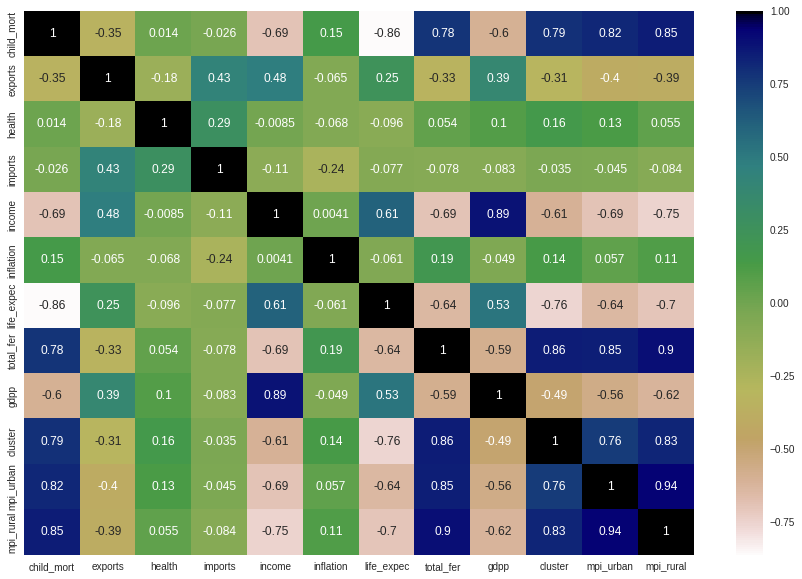
\includegraphics[width=.9\linewidth]{mpi-rural-urban-heatmap}
    \caption{Heatmap with MPI rural and urban}
    \label{fig:mpi-urban-rural-heatmap}
\end{figure}

Also the heatmap output of the country dataset as shown in Figure~\ref{fig:mpi-urban-rural-heatmap} with the newly attached features named MPI urban and MPI rural seems to have a high correlation too. We'll use MPI urban as the DV here. Features that are in high correlation with MPI urban are child mortality, income, life expectancy, total fertility, and GDPP. We'll not use any such features that are highly correlated, and might have multicollinearity between them. Multicollinearity occurs when there are high intercorrelations among two explanatory variables in a multiple regression model.

After that, to uncover the relationship between the dependent variable and the independent variables, a simple linear and multivariate regression model was used for all features (IV) from the original dataset using MPI urban as the DV.

We used the Linear regression statistical method as the next step up after correlation because it can help us predict the value of a variable based on the value of another variable by looking at different data points and plotting a trend line. In this stage, income and GDPP showed high multicollineartiy with MPI urban as, shown in Figure~\ref{fig:linear-income-gdpp}. In contrast, some other features like child mortality, total fertility, life expectancy were showing unequal scatter indicating heteroscedasticity due to the presence of outlier in the data. 

And after working the linear regression, we went for the multivariate
regression. Multivariate regression is an extension of multiple regression, which seeks to
predict the dependent variable with the help of two or more independent variables, helping
us understand the correlation between our dependent and independent variables.

\begin{figure}[!htp]
    \centering
    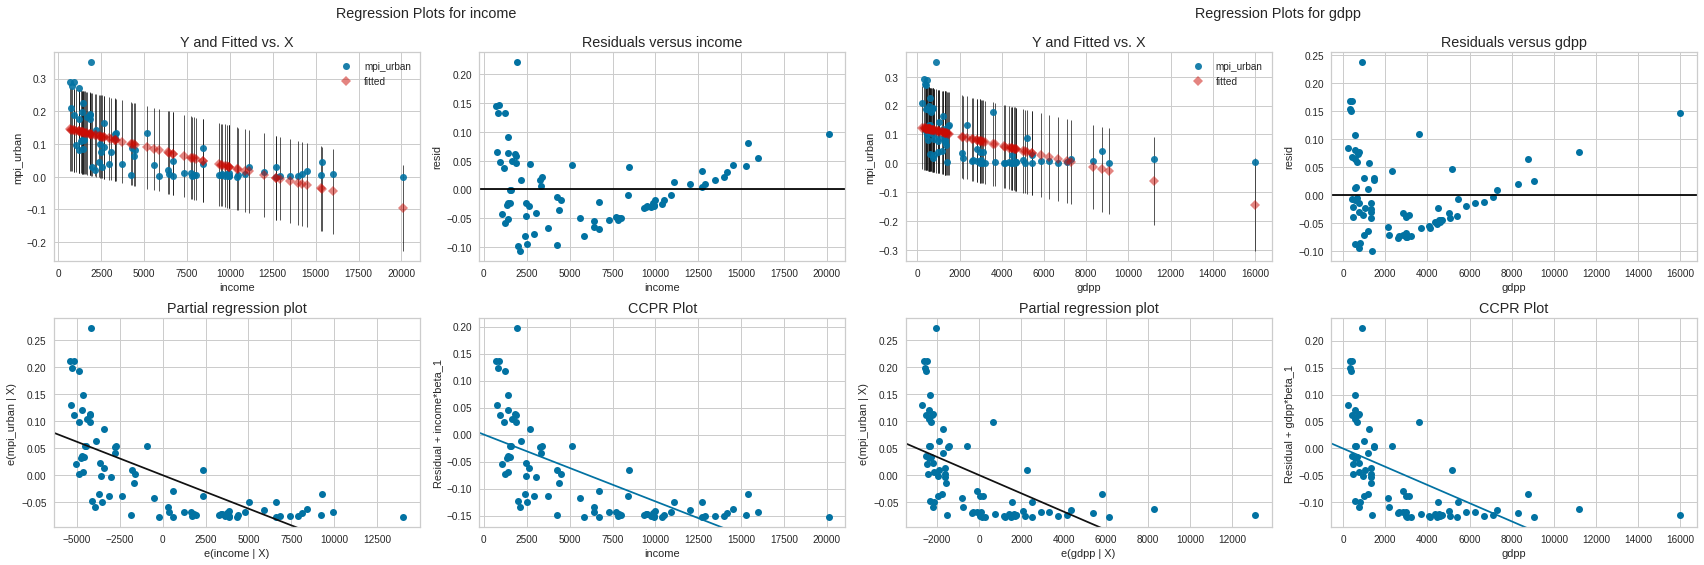
\includegraphics[width=\linewidth]{linear-income-gdpp}
    \caption{Regressions showing high multicollinearity}
    \label{fig:linear-income-gdpp}
\end{figure}

Later we measured the adjusted R-squared values for multivariate regression with all features of the original dataset, which we found to be a good score of \(80\%+\). In this analysis, R-squared indicates the proportion of variance in MPI Urban, explained by the selected features. Accordingly, adjusted R-squared is the revised variant of R-squared that adjusts for the predictor's number in a regression model, making it a better model evaluator and can correlate the variables more efficiently than R-squared. Then we continued measuring the adjusted R-squared value with features with the highest R-squared value found on simple linear regression and got 79\% in the result. Based on the initial correlation analysis of these features, they have a high positive correlation. We've also calculated the value without features with multicollinearity and heteroscedasticity but got only 39\%.

And now, we can apply the findings that we've found so far to narrow our features and run
a new clustering model. We'll incorporate countries listed on clusters 0 and 1 and
consolidate them to work on a different dataset. The features we'll be using to cluster this new
dataset are child mortality, GDPP, and MPI urban. It's because the child mortality rate proved to be a strong indicator for recommending the development aid, the GDP per person is an acknowledged indicator for measuring poverty, and the MPI urban is selected for its capability of capturing the multidimensional proportion of the population in need of aid and the intensity of their deprivations. We had to eliminate the columns that contain the
country information because only the numeric values should be utilized, in this case of
unsupervised learning. After that, we've again continued the processes we've previously
arranged in Section~\ref{sec:mod}. And that resulted in 3 sub-clusters from our previous clusters. In Figure~\ref{fig:subclusters-location}, the Geoplot shows the extracted three
sub-clusters locations in the world.

After completing the sub-clustering exercise as shown in Appendix~\ref{cha:code}, we found the
countries listed on sub-clusters 0 and 1 to have severe conditions in the case of MPI. And based on all the elected parameters named child mortality, MPI, and GDPP, countries in the second sub-cluster were appeared to be in the most critical condition (see Figure~\ref{fig:pairplot-subclusters}).

\begin{figure}[!htp]
  \centering%
  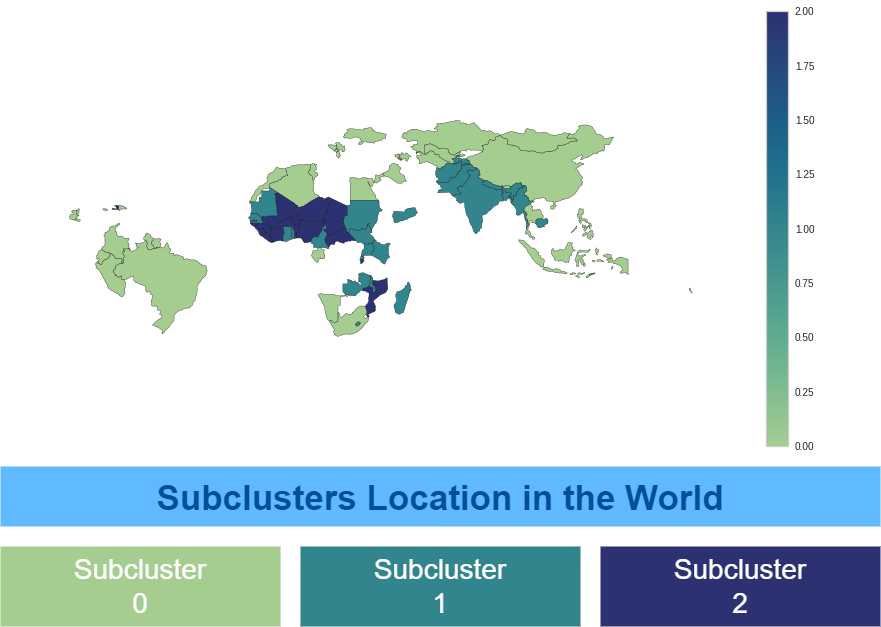
\includegraphics[width=.6\linewidth]{figs/subclusters-location}
  \caption{Sub-clusters location in the world}
  \label{fig:subclusters-location}
\end{figure}

\begin{figure}[!htp]
    \centering
    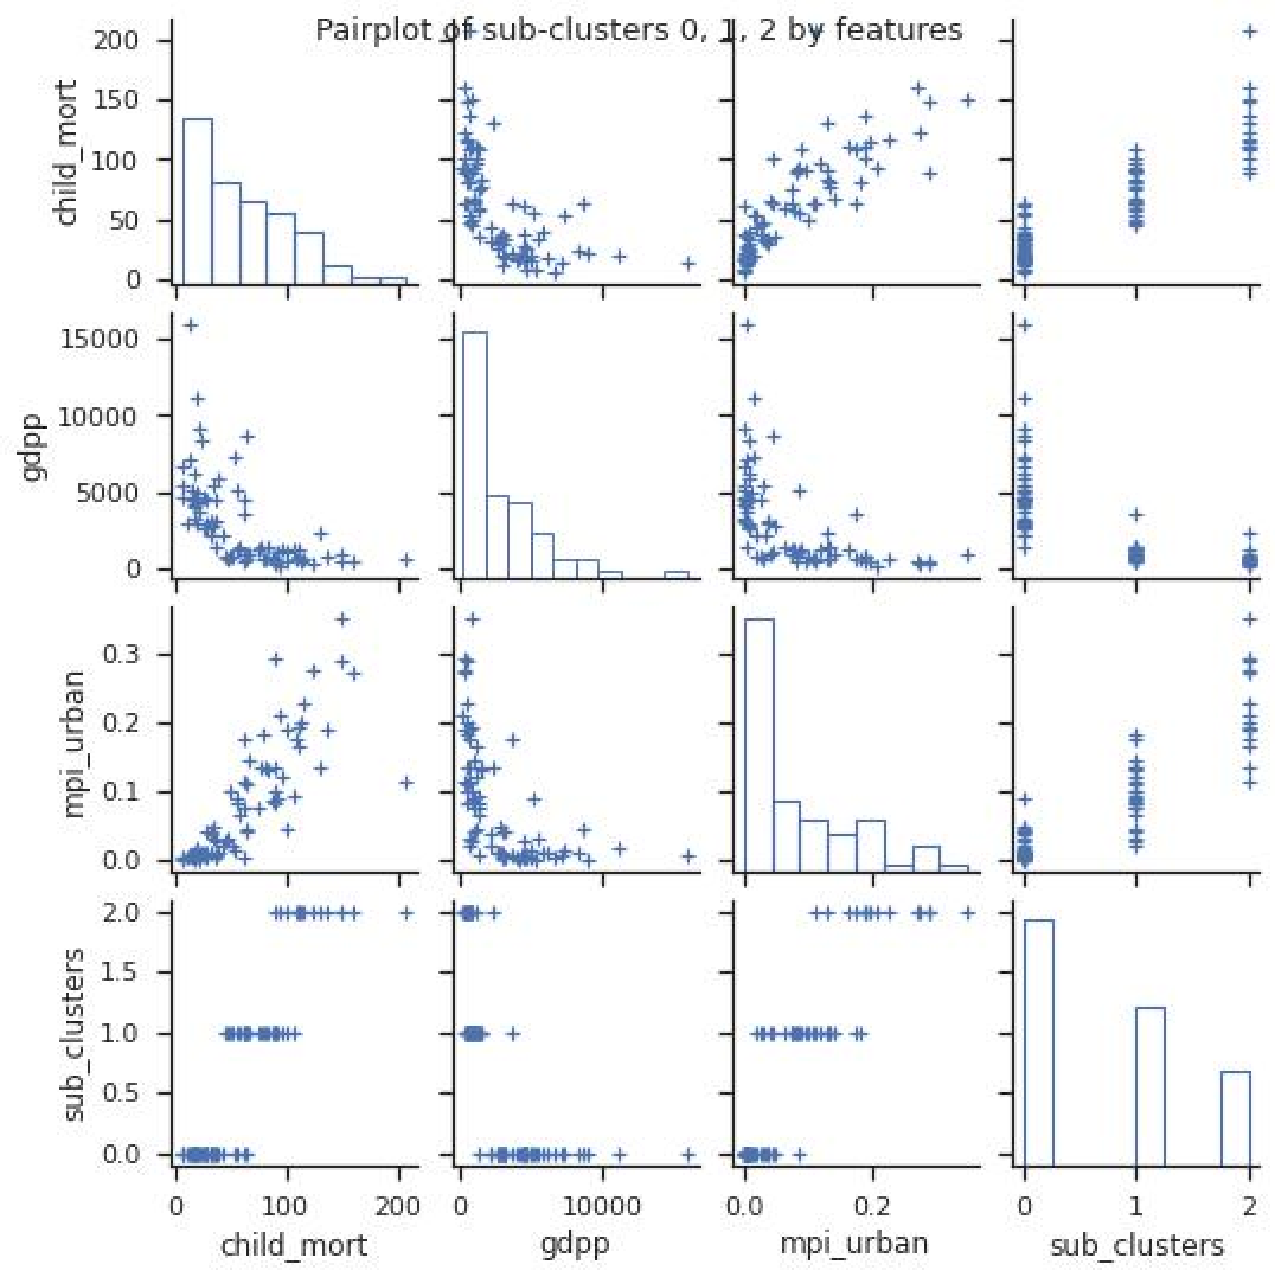
\includegraphics[width=.8\linewidth]{figs/pairplot-subclusters}
    \caption{Pairplot of sub-clusters by features}
    \label{fig:pairplot-subclusters}
\end{figure}

\chapter{Conclusion}
We have developed a possible machine learning modeling approach to making aid allocation decisions based on multidimensional measures of poverty. This approach can enable donors to distribute development assistance considering all the different aspects of scarcity.

In our study, we have used Principal Component Analysis to reduce the variables involved, and then we went for the clustering of countries based on those principal components. After that, we affirmed those factors that play a vital role in deciding the impoverishment of regions. And by centering those factors, we have built clusters of countries. We can also explore further by making sub-clusters depending on what specific fund objectives or donor interests require highlighting. And based on those clusters, we can later identify the list of countries in urgent need of aid. But this list of countries is subject to change because this model is recommended based on factors like the number of chosen components, clusters, unsupervised learning techniques, etc.

However, we believe the clustering method alone to be not sufficient enough to provide a final recommendation. Further exploration is necessary, and that too by appending more features related to the context and constraints that the recommended countries might be facing. To expand the multidimensionality of this analysis, we also need to study and resolve the systemic challenges or issues that could limit or prevent funding, e.g., corruption, political instability, civic society crisis, natural disasters, and other risks. We must develop more suitable criteria for funding allocation decisions from the donor states and agencies. And those indicators should rely on the current context of a country, past the macro indicators. Our shown approach in this study can help guide the necessary actions for this further analysis and detailed exploration.

Overall, this paper argues that for aid to be fully effective, it can no longer be treated as a voluntary, charitable transfer based on traditional monetary indicators of economic development. Instead, aid must be part and parcel of a wider re-distributive agenda meant to protect the basic rights of our fellow human beings. For this to happen, poor people’s voices, needs, and priorities need to be put in the center of the design of aid allocation programs through the help of multidimensional indicators and machine learning algorithms.

\section{Result}
\label{sec:result}

From our findings based on multidimensional aspects of poverty, a list of countries, as shown in Table~\ref{tab:sc012}, were recommended by the system for their grave need of aid (from sub-cluster 0 to 2).

\begin{table}[ht]
  \centering\singlespacing%
  \caption{List of recommended countries for aid\label{tab:sc012}}
  \begin{tabular}{llllll}
    \toprule
    ISO&Name                    &ISO&Name             &ISO&Name        \\\midrule
    BJ &Benin                   &GM &Gambia           &MZ &Mozambique  \\
    BF &Burkina Faso            &GQ &Equatorial Guinea&NE &Niger       \\
    BI &Burundi                 &GW &Guinea-Bissau    &NG &Nigeria     \\  
    CM &Cameroon                &HT &Haiti            &SL &Sierra Leone\\           
    CF &Central African Republic&LR &Liberia          &TD &Chad        \\           
    CI &Côte d'Ivoire           &ML &Mali             &TL &Timmor-Leste\\\bottomrule
  \end{tabular}
\end{table}

But like all machines, every developed system can only be as effective as the people
running them and the data that goes into them. Employing data in machine learning is not a
solution but a tool to be used in the hands of responsible leaders.

\section{Discussion}
As specified in section~\ref{sec:result}, the listed countries recommended by our machine learning model affirm the view of computer algorithms being capable of allocating aid resources based on a constantly updated data-fed system. But surprisingly, there is very little use of this approach in practice, as opposed to politics and international relationships. While in the development field, machine learning is already being used in a wide range of applications, from the traditional supervised methods to predict poverty rates to housing conditions, food security, etc. 

We should start studying and developing novel tools in support of aid and SDGs because traditional monetary indicators of economic development are an unarguably incomplete measure of aid allocation. Also, according to many researchers, development aids are not being as effective as expected because of the sly foreign policies and their dependence on these monetary indicators. From the disingenuous motive behind its provision to its delivery at every stage, there are predicaments. 

It is why future research should concentrate on linking the SDGs with the current aid allocation strategies to find the gaps and expedient areas for improvement in aid allocation strategy using all our digital aptitudes. In accordance, recipient governments also need to reform. Accountability, follow-up, transparency, democracy, and the protection of human rights must all be improved. And the fact that expanding aid allocations for some countries means less funding for others, we must do something about that too. We should start grouping aid into several new types of categories. It will help us begin to test broader and more theoretically driven hypotheses about aid allocation. Furthermore, we must participate in helping donor countries and agencies in making allocation policies and strategies more systematically efficient for it to genuinely impact the lives of all the people in need. 

In conclusion, we must understand that, behind all those studies, numbers, analysis, and statistics are real people with their difficulties and stories. And all those stories aren't a matter of reducing into a single number. Hence we need to start considering human elements in a data-driven system to keep aid allocations effective, as human development is more about giving people the opportunities to live lives they value, and enable them to achieve their destiny. This goes beyond material resources as people also value many other aspects of life. Viewing from this wider set of criteria can help us understand the full picture of dimensions that need consideration. OPHI has been working on identifying many missing dimensions of poverty that deprived people cite as important in their experiences of poverty. If we call attention to these missing dimensions while designing aid distribution strategies and use them as a guide to policy, development aids can help achieve Sustainable Development Goals by 2030.

\appendix%

\makebib % Bibliography

\begin{advisorInfo} 
  WANG Xiaolin, obtained his MSc degree in distributed computing systems in Greenwich
  University, London, UK in 1998. Since 2004, he has been working as a lecturer in Southwest
  Forestry University teaching computer networks, operating systems, and Linux application
  programming related courses.  
\end{advisorInfo}

\begin{acknowledgment}
\begin{center}
 Dedicated to all the great teachers who instilled in me the joy of learning, \\my parents, sisters, and friends.  
\end{center}
\end{acknowledgment}

%%%%% Appendix chapters
\singlespacing
\setlength{\parindent}{0pt}

\chapter{Source code}
\label{cha:code}

\section{Importing}

\subsection{Libraries}

\begin{pythoncode}
#!/usr/bin/python3
import os
import geoplot
import numpy as np
import mapclassify
import pandas as pd
import seaborn as sns
import geopandas as gpd
import plotly.express as px
import statsmodels.api as sm
import matplotlib.pyplot as plt
from sklearn import linear_model
from sklearn.cluster import KMeans
from sklearn.decomposition import PCA
from statsmodels.formula.api import ols
from geopandas import GeoDataFrame as gdf
from sklearn.metrics import silhouette_score
from sklearn.preprocessing import MinMaxScaler
from sklearn.preprocessing import StandardScaler
from yellowbrick.cluster import SilhouetteVisualizer
\end{pythoncode}

\subsection{Datasets}

\begin{pythoncode}
country = pd.read_csv("country.csv") # https://github.com/evonshahriar/grab/blob/main/country.csv
n_mpi = pd.read_csv("n_mpi.csv") # https://github.com/evonshahriar/grab/blob/main/n_mpi.csv
sn_mpi = pd.read_csv("sn_mpi.csv") # https://github.com/evonshahriar/grab/blob/main/sn_mpi.csv
\end{pythoncode}

\section{Preprocessing}

To see data features.

\begin{pythoncode}
country.head() 
#n_mpi.head()
#sn_mpi.head()
\end{pythoncode}

To check for missing values.

\begin{pythoncode}
country.isnull().sum()
\end{pythoncode}

To check for duplicate values.

\begin{pythoncode}
format(len(country[country.duplicated()]))
\end{pythoncode}

To see data distribution of features. 

\begin{pythoncode}
plt.figure(figsize=(14, 7))
plt.title(
    "Child Mortality\n(Death of children under 5 years of age per 1000 live births)"
)
cm = sns.histplot(country["child_mort"])
cm.set_facecolor("#f0ffff")
\end{pythoncode}

To check the correlation. 

\begin{pythoncode}
plt.figure(figsize=(14, 9))
plt.title("Pearson correlation coefficient")
sns.heatmap(
    country.corr(method="pearson", min_periods=1), annot=True, cmap="Greens"
)  # change method to 'kendall' or 'spearman' to see those correlation outputs
\end{pythoncode}

To eliminate columns without numeric value.

\begin{pythoncode}
country_n = country.drop(["country"], axis=1)
country_n.head()
\end{pythoncode}

To scale using MinMaxScaler.

\begin{pythoncode}
columns = country_n.columns
scaler = MinMaxScaler()
country_minmax = scaler.fit_transform(country_n)
df_minmax = pd.DataFrame(data=country_minmax, columns=columns)
df_minmax
\end{pythoncode}

To scale using StandardScaler.

\begin{pythoncode}
columns = country_n.columns
scaler = StandardScaler()
country_standard = scaler.fit_transform(country_n)
df_standard = pd.DataFrame(data=country_standard, columns=columns)
df_standard
\end{pythoncode}

To compare the scaling methods. 

\begin{pythoncode}
# StandardScaler
plt.scatter(
    df_standard["gdpp"], df_standard["child_mort"], color="green"
)  # use 'df_minmax' to compare with the MinMaxScaler
plt.scatter
plt.title(
    "StandardScaler\n(Standardized the data feature by subtracting the mean and then scales to unit variance)"
)
plt.xlabel("GDP per capita")
plt.ylabel("Child mortality")
\end{pythoncode}

Principal Component Analysis.

\begin{pythoncode}
# Using the StandardScaler data
cap = PCA()
cap.fit(df_standard)  # 'df_minmax' for using the MinMaxScaler data
cap_data_standard = cap.transform(df_standard)  # use 'df_minmax' for MinMaxScaler
percent_var = np.round(cap.explained_variance_ratio_ * 100, decimals=1)
labels = ["PC" + str(x) for x in range(1, len(percent_var) + 1)]
plt.bar(x=range(1, len(percent_var) + 1), height=percent_var, tick_label=labels)
plt.ylabel("% of Explained Variance")
plt.xlabel("Principal Component")
plt.title("StandardScaler (Scree Plot)")
plt.show()
cap_df_standard = pd.DataFrame(cap_data_standard, columns=labels)
plt.scatter(cap_df_standard.PC1, cap_df_standard.PC2)
plt.title("StandardScaler (PCA)")
plt.xlabel("PC1 - {0}%".format(percent_var[0]))
plt.ylabel("PC2 - {0}%".format(percent_var[1]))
\end{pythoncode}

To data-frame the principal components 1, 2, 3, and 4 into one dataset.

\begin{pythoncode}
data = pca_df_standard.drop(["PC5", "PC6", "PC7", "PC8", "PC9"], axis=1)
\end{pythoncode}

\section{Modeling}

To setup the k-means clustering model.

\begin{pythoncode}
kmc = KMeans(
    n_clusters=3, init="random", n_init=10, max_iter=300, tol=1e-4, random_state=0
)
\end{pythoncode}

To run the model with different datasets and add the cluster in a new column. 

\begin{pythoncode}
preminmax = km.fit_predict(df_minmax)
df_minmax["cluster"] = preminmax
prestandard = km.fit_predict(df_standard)
df_standard["cluster"] = prestandard
precountry = km.fit_predict(data)
country_n["cluster"] = precountry
\end{pythoncode}

To find the distortions (SSE) of different clusters using the Elbow method.

\begin{pythoncode}
# For dataframe scaled with StandardScaler
elsse = []
for i in range(1, 11):
    km = KMeans(
        n_clusters=i, init="random", n_init=10, max_iter=300, tol=1e-04, random_state=0
    )
    km.fit(
        df_standard
    )  # change the 'df_standard' to 'df_minmax'/'country_n'/other to calculate the sse for those datasets
    sse.append(km.inertia_)
plt.plot(range(1, 11), sse, marker="o")
plt.xlabel("Number of clusters")
plt.ylabel("Sum of Squared Errors")
plt.show()
\end{pythoncode}

To find the Silhouette scores of the cluster.
\# With Standardized data

\begin{pythoncode}
silscore = silhouette_score(
    df_standard, km.labels_, metric="euclidean"
)  # change the 'df_standard' to other df names to check the score for those dataframes
print("Silhouette Score: %.2f" % score)
\end{pythoncode}
% 

\section{Analyzing}

To visualize the clusters by features.

\begin{pythoncode}
# Visualization for data with StandardScaler
sns.get_dataset_names()
sns.load_dataset("penguins")
sns.pairplot(
    df_standard, hue="cluster"
)  # change the 'df_standard' to other df names to check the score for those dataframes
plt.suptitle(
    "Pairplot of clusters by feature (Scaled data with StandardScaler)", size=15
)
\end{pythoncode}

To see the clusters description with their features mean. 

\begin{pythoncode}
clusters = pd.pivot_table(data, index=["cluster"])
clusters
\end{pythoncode}

To see the countries each cluster hold.

\begin{pythoncode}
cluster_0 = data.loc[data["cluster"] == 0]
cluster_0.country.unique()
# cluster_1 = data.loc[data['cluster'] == 1]
# cluster_1.country.unique()
# cluster_2 = data.loc[data['cluster'] == 2]
# cluster_2.country.unique()
\end{pythoncode}

To see the clusters location in the world. 

\begin{pythoncode}
world = gpd.read_file(gpd.datasets.get_path("naturalearth_lowres"))
world_countries = world.copy()
world_countries.rename(columns={"name": "country"}, inplace=True)
world_countries.head()
world_data = pd.merge(country, world_countries, on="country", how="inner")
world_data = gdf(world_data)
cluster = world_data["cluster"]
geoplot.choropleth(world_data, hue=cluster, cmap="crest", figsize=(16, 8), legend=True)
\end{pythoncode}

\section{Finalizing}

To drop the features with high correlation. 

\begin{pythoncode}
# For the country dataset
country_r = country.drop(["country", "life_expec", "total_fer", "income"], axis=1) 
country_r.head() 
\end{pythoncode}

To again scale the reduced dataset.

\begin{pythoncode}
# For standard scaling
columns = country_r.columns
scaler = StandardScaler()
country_rs = scaler.fit_transform(country_r)
df_r = pd.DataFrame(data=country_rs, columns=columns)
\end{pythoncode}

To compute the clusters in the reduced scaled datasets.

\begin{pythoncode}
pre_r = km.fit_predict(df_r)
pre_r
\end{pythoncode}

To add the cluster column to the df and calculate the SSE.

\begin{pythoncode}
df_r["cluster"] = pre_r
sse_r = []
for i in range(1, 11):
    km = KMeans(
        n_clusters=i, init="random", n_init=10, max_iter=300, tol=1e-04, random_state=0
    )
    km.fit(df_r)
    sse_r.append(km.inertia_)
plt.plot(range(1, 11), sse_r, marker="o")
plt.xlabel("Number of clusters")
plt.ylabel("SSE")
plt.show()
\end{pythoncode}

To see the pairplot for a particular cluster by its features.

\begin{pythoncode}
c2 = data[data.cluster == 2]
sns.get_dataset_names()
sns.load_dataset("penguins")
sns.pairplot(
    c2,
    height=1.5,
    plot_kws=dict(marker="+", linewidth=1.2),
    diag_kws=dict(fill=False),
)
plt.suptitle("Pairplot of cluster 2 by features", size=16)
\end{pythoncode}

To incorporate more new features into the dataframe from other datasets. 

\begin{pythoncode}
# E.g. To append features from the 'n_mpi' dataset
ns_mpi = n_mpi.drop(
    [
        "ISO",
        "Headcount Ratio Urban",
        "Intensity of Deprivation Urban",
        "Headcount Ratio Rural",
        "Intensity of Deprivation Rural",
    ],
    axis=1,
)

ns_mpi.rename(
    columns={"Country": "country", "MPI Urban": "mpi_urban", "MPI Rural": "mpi_rural"},
    inplace=True,
)

zippie = pd.merge(country, ns_mpi, on="country", how="inner")
zippie.head()
\end{pythoncode}

To do linear regression between a dependent variable and an independent variable. 

\begin{pythoncode}
reg = linear_model.LinearRegression()
lm = ols(
    "mpi_urban ~ income", country=combined
).fit()  # To find others, change mpi_urban and income with the desired DV and IV
print(lm.summary())
fig = plt.figure(figsize=(14, 9))
fig = sm.graphics.plot_regress_exog(lm, "income", fig=fig)
\end{pythoncode}

To do multivariate regression and find the adjusted R-squared between a DV and multiple IV.

\begin{pythoncode}
reg.fit(
    combined[["exports", "health", "imports", "inflation", "gdpp"]], combined.mpi_urban
)
ars = 1 - (
    1
    - reg.score(
        combined[["exports", "health", "imports", "inflation", "gdpp"]],
        combined.mpi_urban,
    )
) * (len(combined.mpi_urban) - 1) / (
    len(combined.mpi_urban)
    - combined[["exports", "health", "imports", "inflation", "gdpp"]].shape[1]
    - 1
)
\end{pythoncode}

To do clustering of clusters for making new sub-clusters. 

\begin{pythoncode}
sc = cluster_0.append(cluster_1, ignore_index=True)
nsc_mpi = pd.merge(sc, ns_mpi, on="country", how="inner")

nsc_mpi.head()

scd = nsc_mpi.drop(
    [
        "country",
        "cluster",
        "exports",
        "health",
        "imports",
        "income",
        "inflation",
        "life_expec",
        "total_fer",
        "mpi_rural",
    ],
    axis=1,
)


columns = scd.columns

scaler = StandardScaler()

r_scd = scaler.fit_transform(scd)

sub_cluster = pd.DataFrame(data=r_scd, columns=columns)
sub_cluster
\end{pythoncode}

To again compute the clusters, and then add the assigned cluster columns to the data frame.

\begin{pythoncode}
sc_km = KMeans(
    n_clusters=3, init="random", n_init=10, max_iter=300, tol=1e-4, random_state=0
)
pre_subc = km2.fit_predict(sub_cluster)
sub_cluster["sub_clusters"] = pre_subc
sub_cluster.head()
\end{pythoncode}

To add this clustered column to the original dataset and then eliminate the columns with country infornations.

\begin{pythoncode}
scm["sub_clusters"] = pred_subc.tolist()
scn = scm.drop(
    [
        "exports",
        "health",
        "cluster",
        "imports",
        "income",
        "inflation",
        "life_expec",
        "total_fer",
        "mpi_rural",
    ],
    axis=1,
)
\end{pythoncode}

To see the pair plot of the subclusters by features.

\begin{pythoncode}
sns.get_dataset_names()
sns.load_dataset("penguins")
sns.pairplot(
    sub_cluster_narrow,
    height=1.9,
    plot_kws=dict(marker="+", linewidth=1.2),
    diag_kws=dict(fill=False),
)
plt.suptitle("Pairplot of sub-clusters 0, 1, 2 by features", size=13)
\end{pythoncode}

To check the country's name each sub-cluster holds.

\begin{pythoncode}
# To check the countries listed on sub-cluster 2
sub_cluster_2 = scn.loc[scn["sub_clusters"] == 2]
sub_cluster_2.country.unique()
\end{pythoncode}

To look for additional countries in need of aid from other clusters and compare.

\begin{pythoncode}
plt.figure(figsize=[15, 9])
plt.barh(
    sub_cluster_0["country"],
    sub_cluster_0["mpi_urban"],
    label="MPI urban",
    color="r",  # change 'sub_cluster_0' to other subclusters name and change the 'mpi_urban' to other features name for seeing the respective plots
)
plt.legend()
plt.xlabel("MPI")
plt.ylabel("Countries")
plt.title("MPI by Country for Sub-cluster 0")
plt.show()
\end{pythoncode}
After concluding this phase, the comparison will help the donors and aid agencies to find a specific number of clusters with country's names that have the most critical measures in selected dimensions and guide make aid allocation plans accordingly.
\end{document}

%%% Local Variables:
%%% mode: latex
%%% TeX-master: t
%%% End:
